%\documentclass[]{jsarticle}

%\usepackage[dvipdfmx]{graphicx}
%\usepackage[dvipdfmx]{color}

%\usepackage{amsmath, amssymb}
%\usepackage{mathtools}
%\usepackage{cancel}
%\usepackage{cases}
%\usepackage{bm}

%\usepackage{here}
%\usepackage{colortbl}

%\begin{document}

%----------ここから-------------------
%----------ミューオンビーム-------------------
\section{実験方法}

\subsection{MLF ミューオンビーム}

\subsubsection{加速器科学インターンシップの利用}
KEK が学部3 回生以上を対象に行っている加速器科学インターンシップを利用することにより,ロシアの実験チームの $g - 2$ Beam Profiling Monitor に関する実験のパラサイト実験という形でMLF ミューオンビームを利用できることを知った.ミューオンビームの性能を踏まえて可能な測定量および測定方法を考え実験の準備を行い,そのインターンシップを用いて実際のMLF ミューオンビームを用いて測定を行った.

 \subsubsection{表面ミューオン}
 MLF では炭素原子核に高エネルギーの陽子を衝突させることによってパイオンを生成し,パイオンが崩壊して得られるミューオンを利用している.炭素標的から飛び出したパイオンが超伝導ソレノイド磁石内部で崩壊することによって得られるミューオンは崩壊ミューオンと呼ばれるが,今回利用したのは炭素標的の表面に静止した$\pi^{+}$ の崩壊によって得られる$\mu ^{+}$ で,これは表面ミューオンと呼ばれる.この表面ミューオンは静止したパイオンから生じているため 100~\% のスピン偏極を持っており,非常にエネルギーが低く一定である(運動エネルギーが4.1~MeV)という特徴を有する.表面ミューオンがスピン偏極を持つのは弱い相互作用による崩壊で生じる際に,ニュートリノはヘリシティーが左巻きのもののみが結合することに由来する.なお炭素標的の表面で静止した$\mu^-$ は原子核に捕獲されるため,取り出すことはできない.

表面ミューオンビームラインの性能は表~\ref{muon1} のとおりで,シングルバンチ(短時間のミューオンの集まり)のミューオンビームが$25~\mathrm{Hz}$ でやってくる.ビームの広がりのプロファイルは図~\ref{muon2} のとおりである.%要表記確認

\begin{figure}[H]
\centering
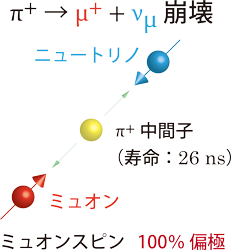
\includegraphics[width=0.4\textwidth]{figure/hayakawa/decay_pion.png}
\caption{$\pi^{+}$ 中間子の崩壊\cite{aboutmuon}}
\end{figure}

\begin{table}[H]
\caption{表面ミューオンビームラインの性能}
\label{muon1}
\centering
\begin{tabular}{cc}\toprule
ビームエネルギー & 4.1~MeV \\ \midrule
侵入長 & $\sim$ 0.2~mm \\ \midrule
エネルギー分布 & $\sim$ 15~\% \\ \midrule
パルス幅 (FWHM) & $\sim$ 100~ns \\ \midrule
ビームサイズ & 30~mm $\times$ 40~mm \\ \midrule
ビーム強度 & 3 $\times$ $10^7~/\mathrm{s}$ \\ \midrule
ポート数 & 2 \\ \bottomrule
\end{tabular}
\end{table}
   
\begin{figure}[H]
\centering
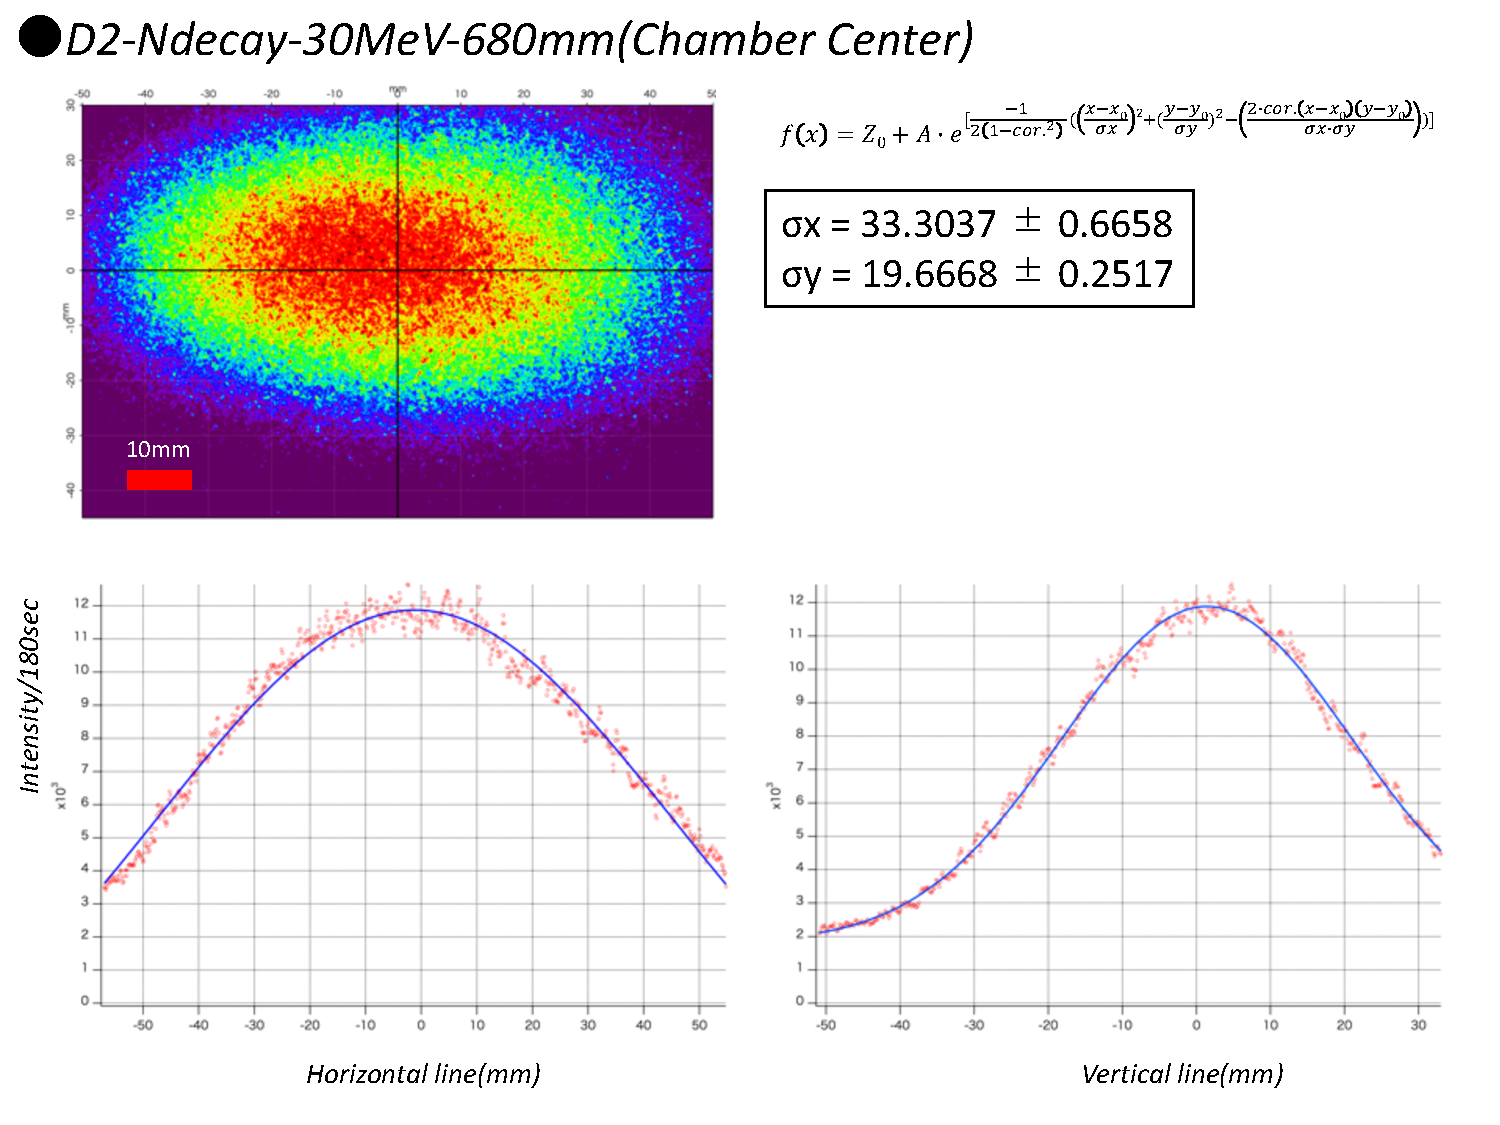
\includegraphics[width=0.8\textwidth]{figure/hayakawa/profile.pdf}
\caption{ミューオンビームの広がり(単位:$\mathrm{mm}$)}
\label{muon2}
\end{figure}

\subsection{測定量と検出器}

\subsubsection{実験概要}

今回の実験ではミューオンの寿命,ミッシェルパラメータ,$g$ 因子を測定する.基本的な実験の流れとしては,
\begin{itemize}
\item ビームラインから $\mu ^{+}$ が出て来る
\item ターゲットに止められた $\mu ^{+}$ が $e^{+}$ に崩壊する
\item 検出器で時間情報・エネルギー情報を測定する
\end{itemize}
という順序になる.測定の時間情報は寿命と$g$ 因子の測定,エネルギー情報はミッシェルパラメータの測定と各解析に対して独立に必要である.そのためにそれぞれの測定を中心に行う検出器として,時間分解能に優れたプラスチックシンチレータ(PS) 検出器および,エネルギー分解能に優れたNaI シンチレータ検出器の二種類の検出器を作成した.    
\begin{figure}[H]
\centering
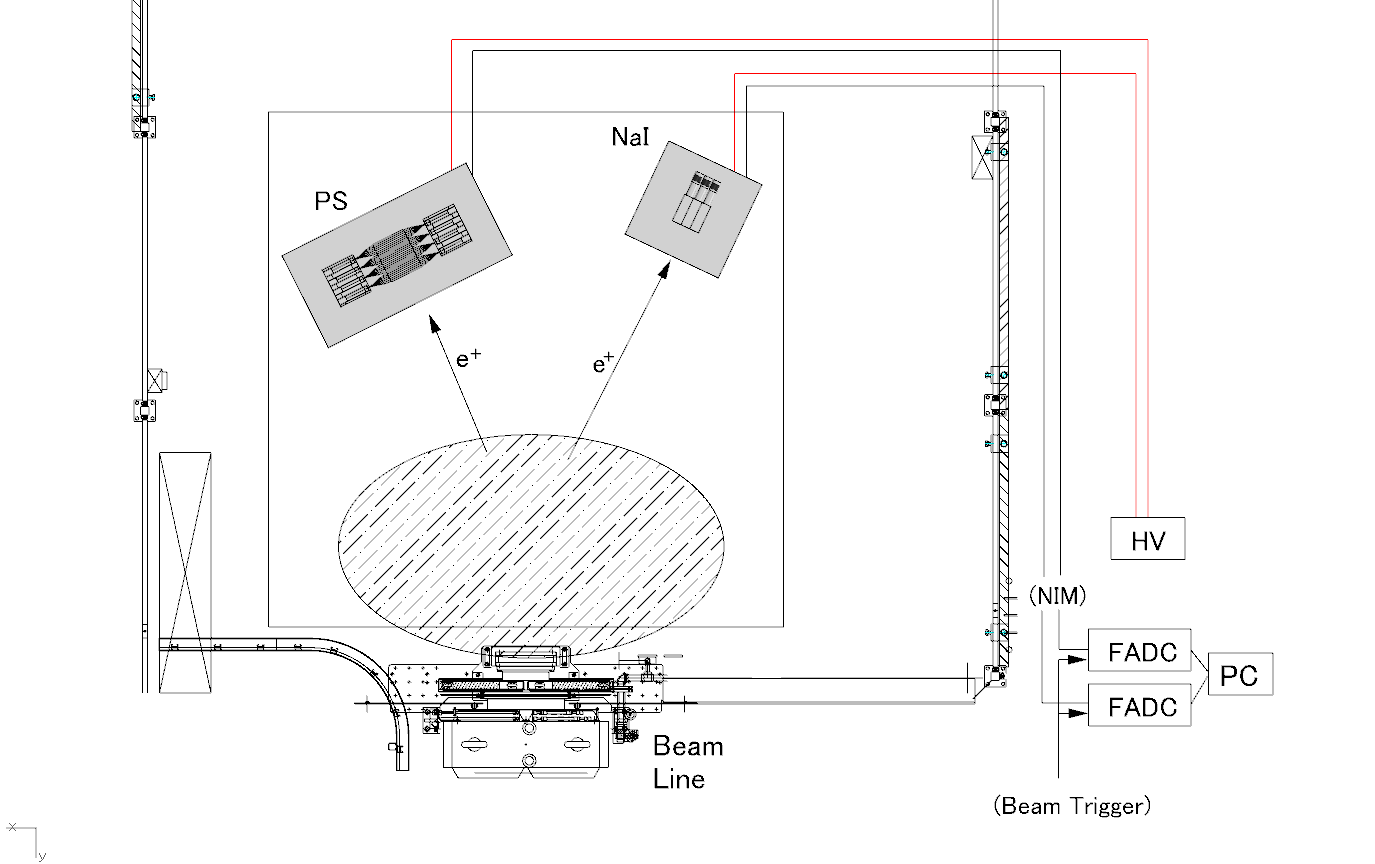
\includegraphics[width=1\textwidth]{figure/hayakawa/lifetime.png}
\caption{実験概要}
\end{figure}

\subsubsection{検出器サイズの見積}

図 \ref{PS_sim} はGeant4 で行ったPS 検出器の体積シミュレーションである.検出器サイズの縦横は $20~\mathrm{cm}$ で固定し,奥行きを $20~\mathrm{cm}$ から$24~\mathrm{cm}$ まで変化させた直方体状のプラスチックシンチレータに測定すべき最大のエネルギーである$50~\mathrm{MeV}$ の陽電子を入射させた.その際に検出器に落としたエネルギーをヒストグラムに示している.奥行きが$24~\mathrm{cm}$ 以下では$50~\mathrm{MeV}$ より下にピークが存在し,電磁シャワーが寸法内に収まらず陽電子のエネルギー充分に検出器に落とせていないことが分かる.一方,奥行きを$24~\mathrm{cm}$ 以上に増やしても,漏れるエネルギーが光子によるものの影響のためほとんど落とすエネルギーは変わらない.つまりこれ以上大きくしても効率が悪く,また基本的には$50~\mathrm{MeV}$ 程度のエネルギーを落としているため,奥行きは$24~\mathrm{cm}$ あれば十分であると決定した.
\begin{figure}[H]
\centering
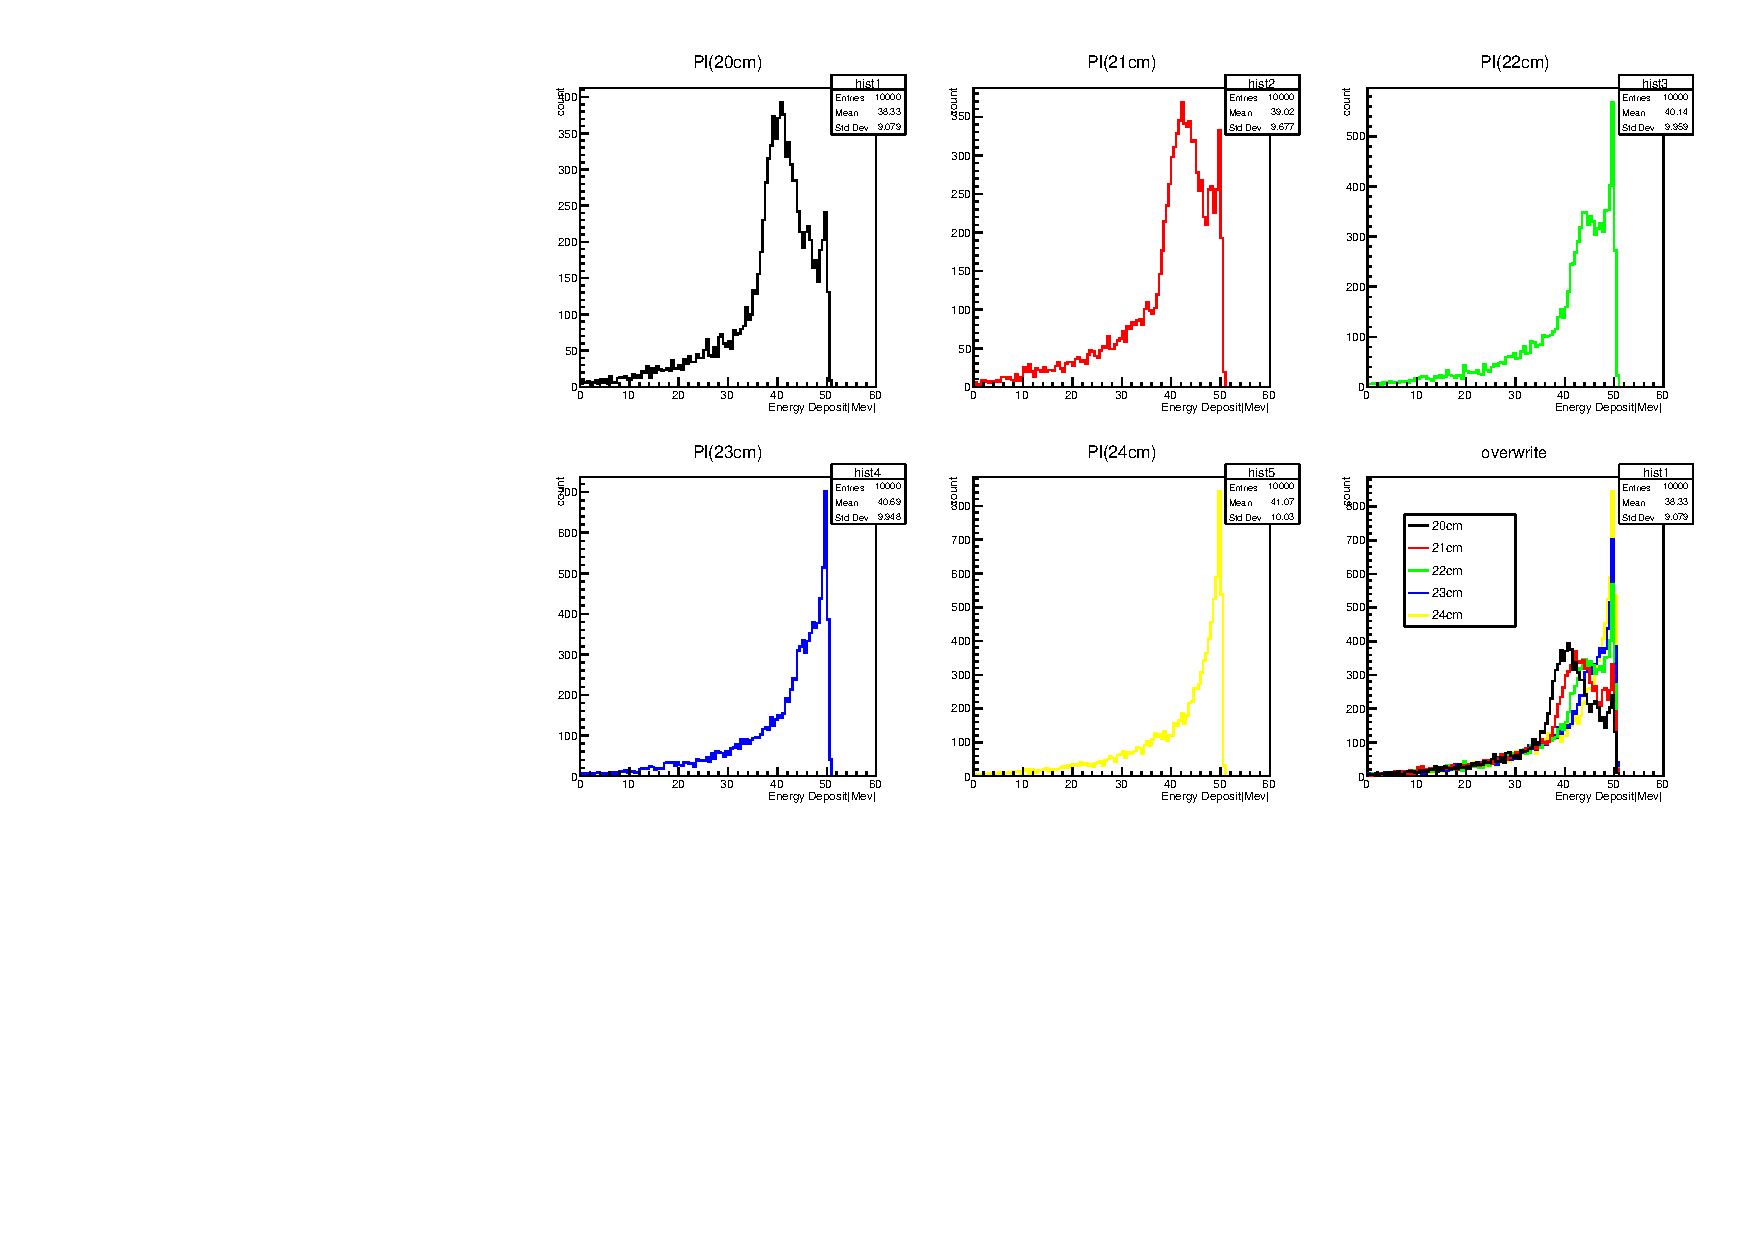
\includegraphics[width=0.6\textwidth,angle=-90]{figure/hayakawa/pl_20_24.pdf}
\caption{PS検出器の体積シミュレーション}
\label{PS_sim}
\end{figure}

図 \ref{NaI_sim} はNaI 検出器の体積シミュレーションである.NaI は光電子増倍管 (PMT) の接続された既製品を利用したため,既製品をどのように並べるべきか確認するために縦横の幅を変えながら同様のシミュレーションを行った.

\begin{figure}[H]
\centering
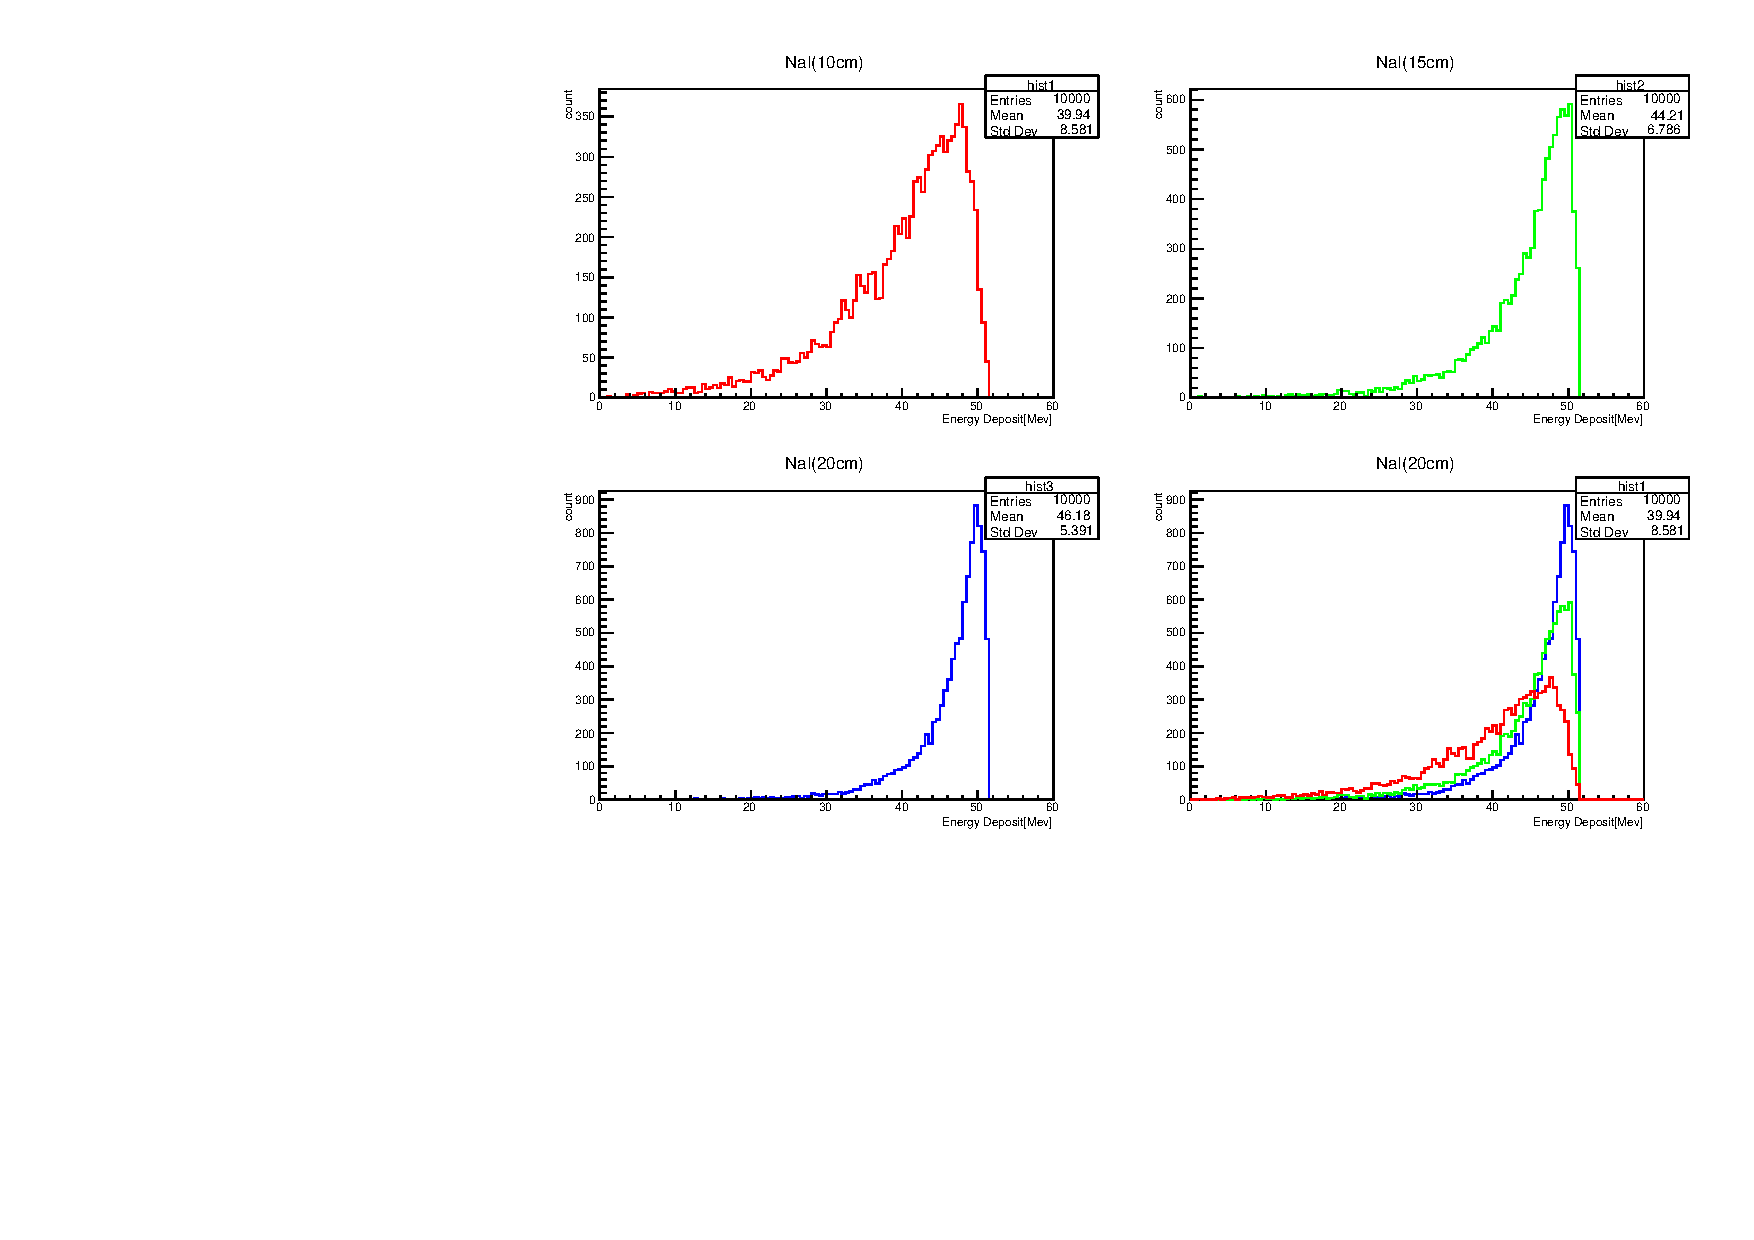
\includegraphics[width=0.55\textwidth,angle=-90]{figure/hayakawa/NaI_10_20.pdf}
\caption{NaI 検出器の体積シミュレーション}
\label{NaI_sim}
\end{figure}

\subsection{検出器の製作}

\subsubsection{PS 検出器の製作}
光ファイバー読み出しの板を並べることで,縦横$20~\mathrm{cm}$ ,奥行き$24~\mathrm{cm}$ の体積のPS 検出器を作成した.

\begin{figure}[H]
\centering
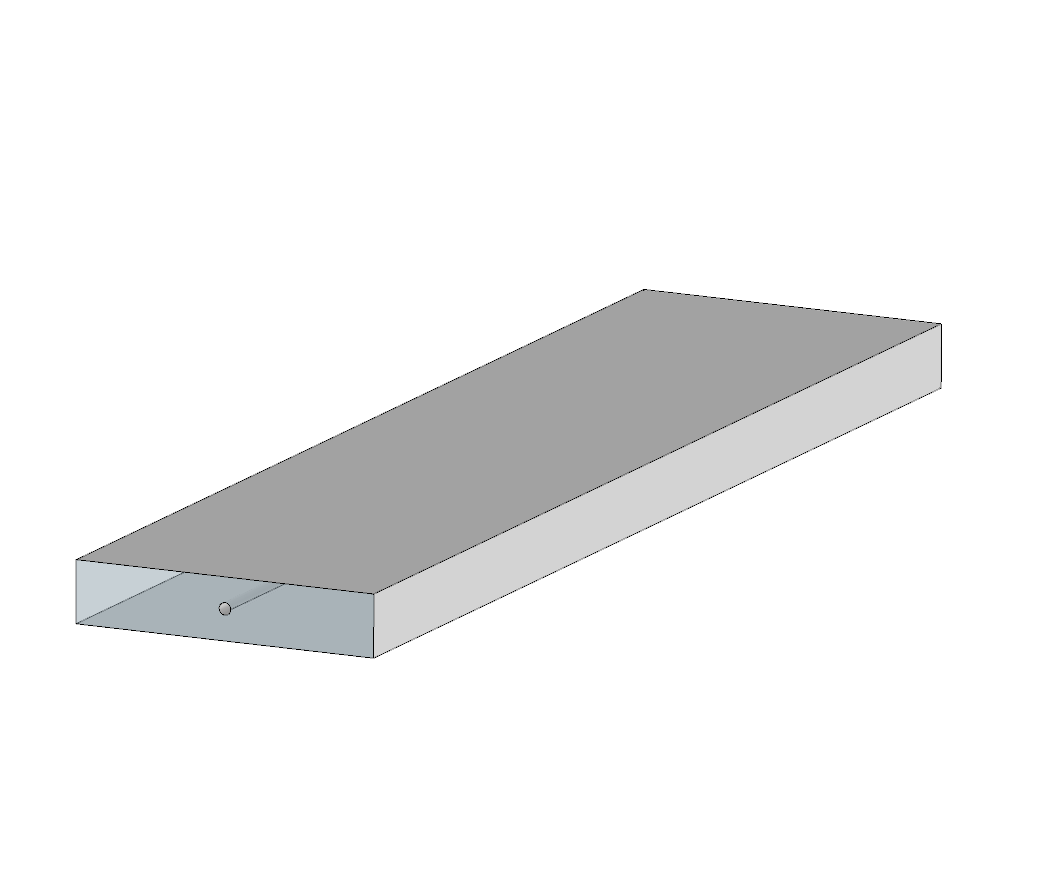
\includegraphics[width=0.3\textwidth]{figure/hayakawa/psmd.png}
\caption{PS 板}
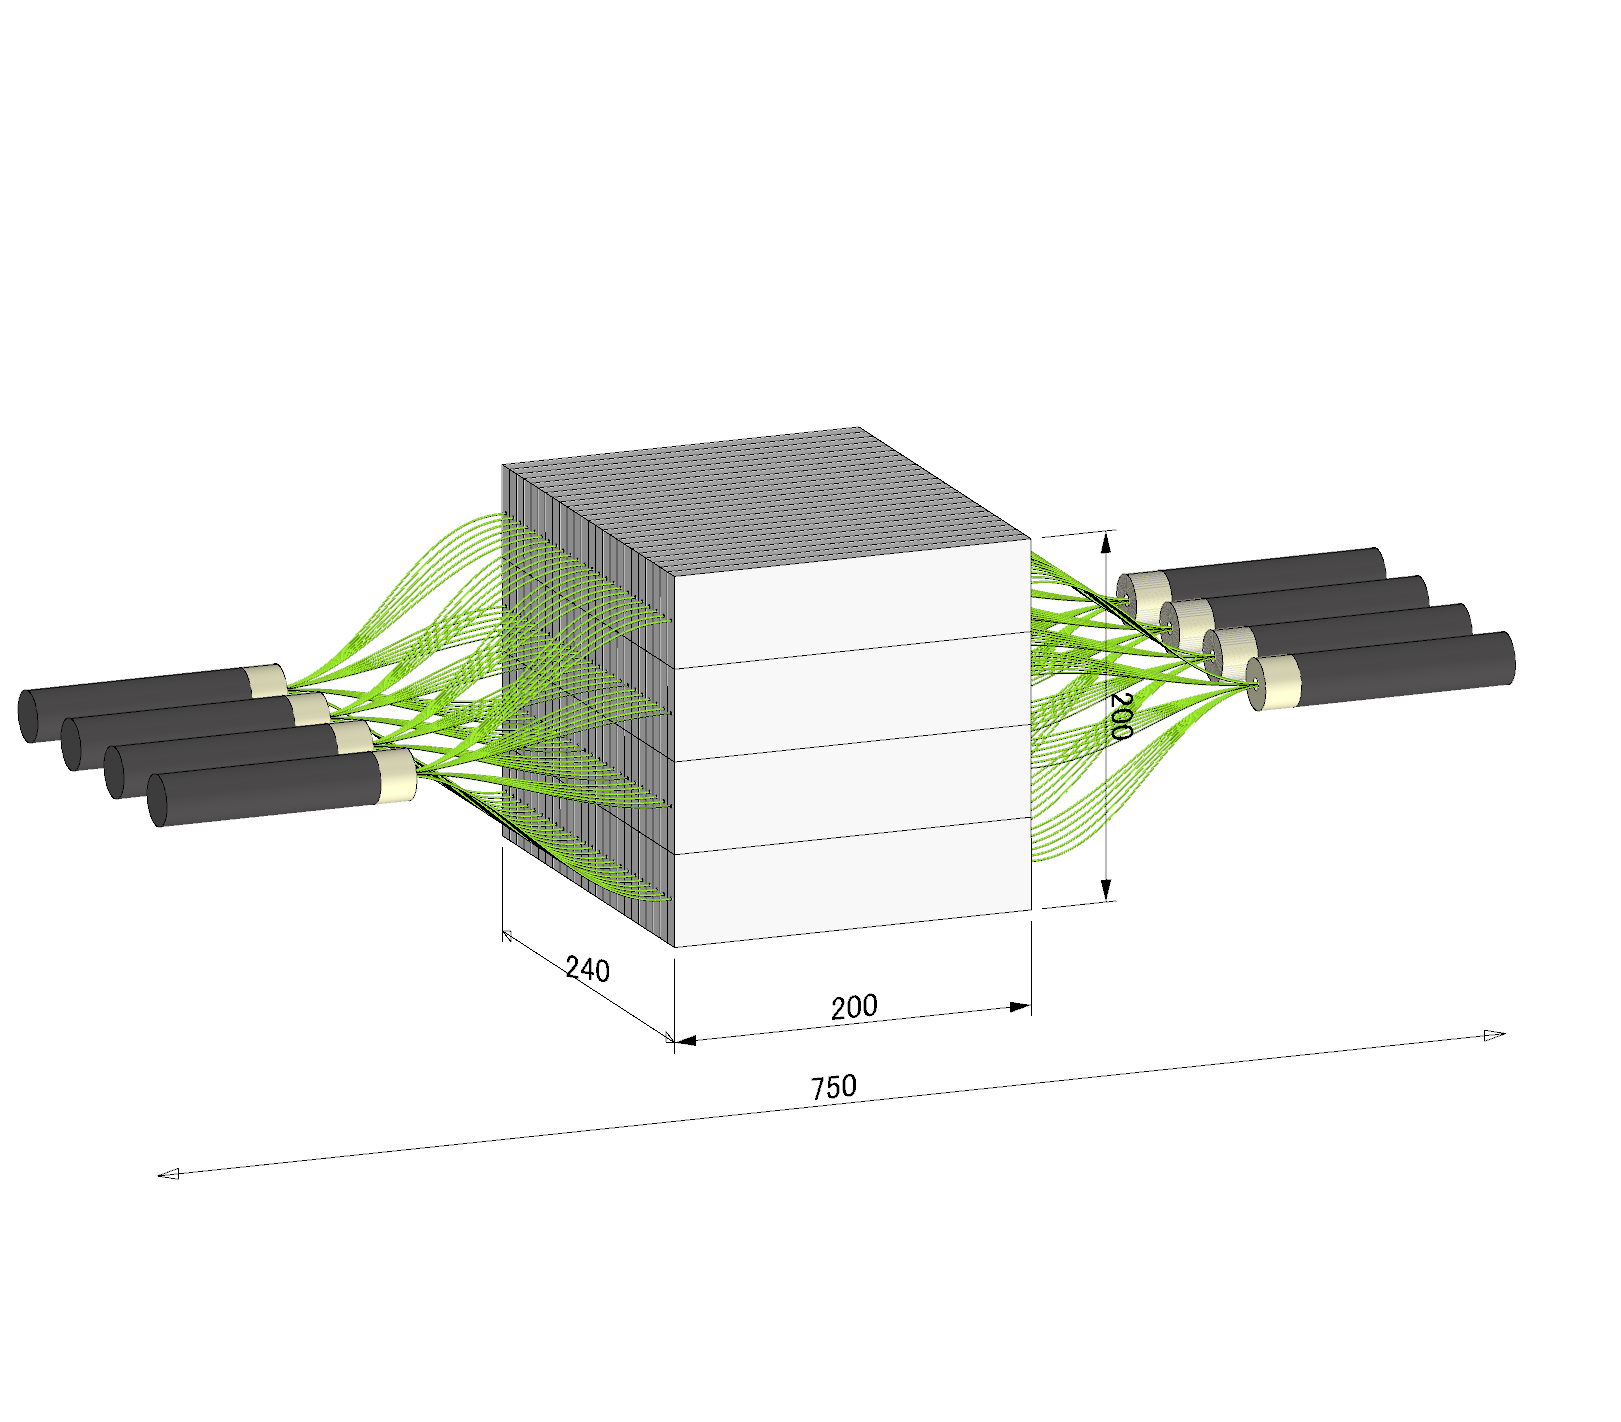
\includegraphics[width=0.8\textwidth]{figure/hayakawa/p7.png}
\caption{PS 検出器寸法}
\label{PS_sunpou}
\end{figure}

以下の順序で検出器を作成した.
\begin{itemize}
\item 厚み$6~\mathrm{cm}$ に束ねたものを$4$ セット作成した
\item 光ファイバーの片端をクッキーを用いて光学セメントで固定した
\begin{figure}[H]
\centering
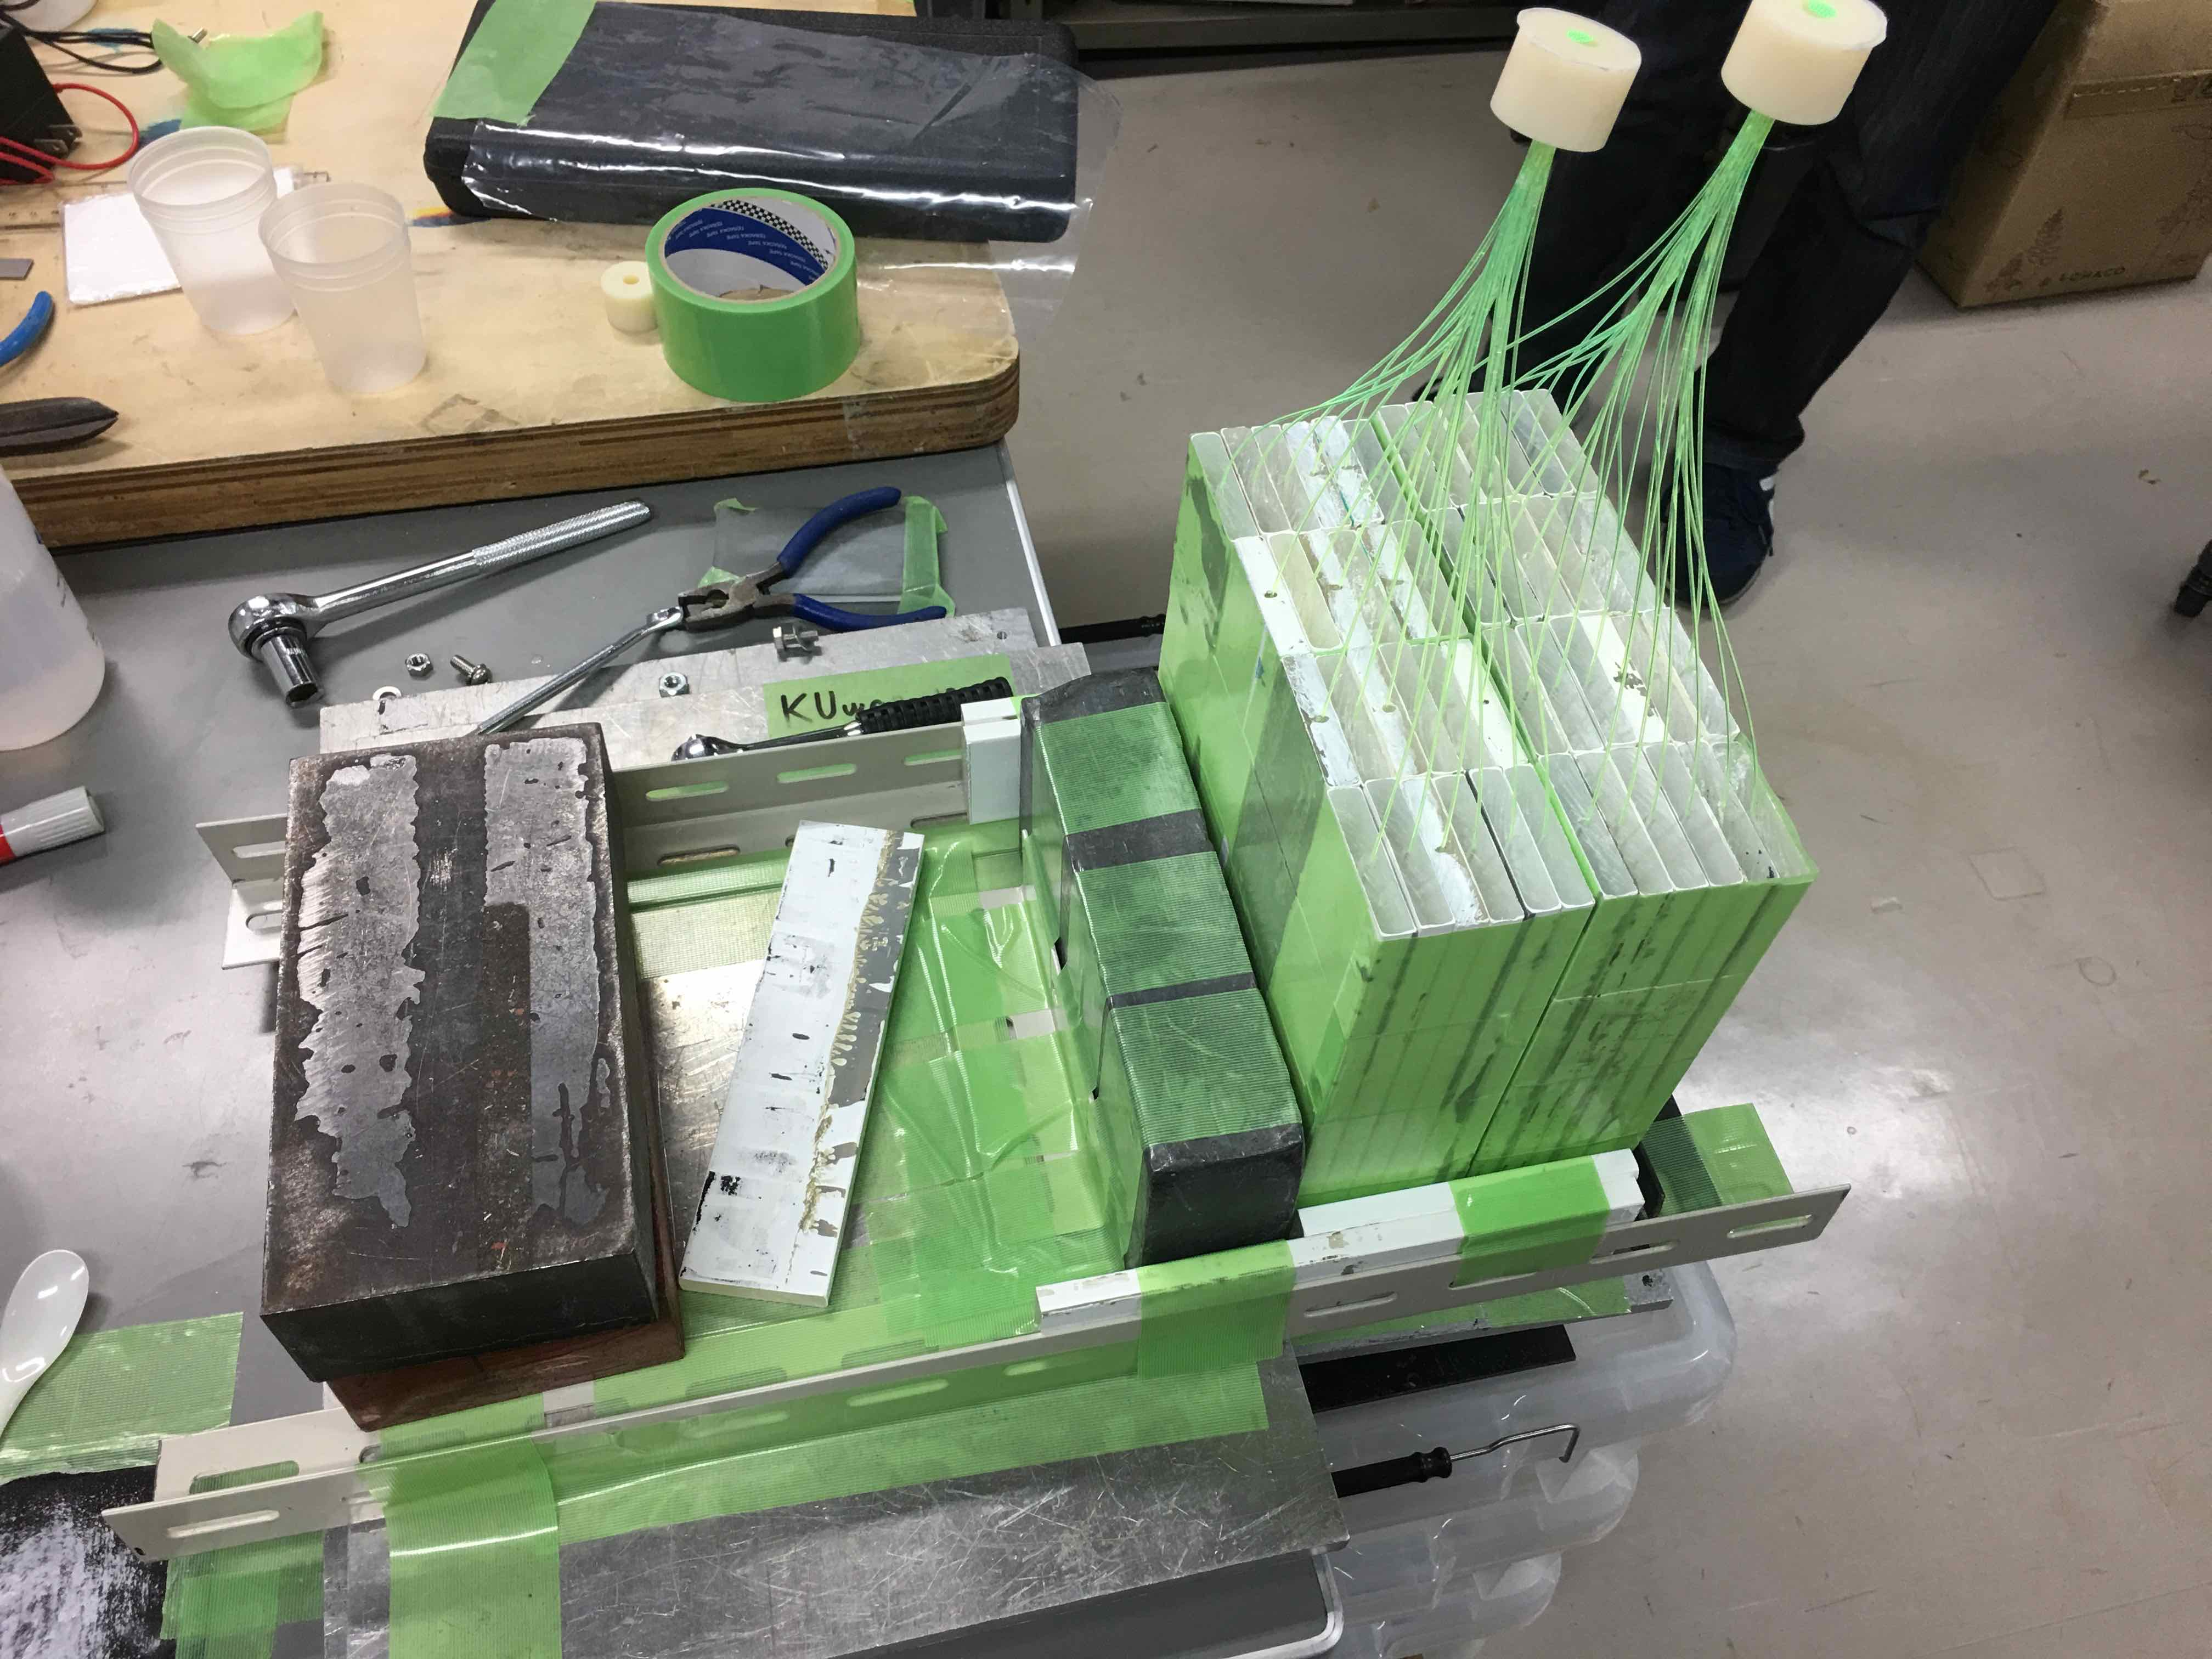
\includegraphics[width=0.5\textwidth]{figure/hayakawa/ps_kotei.jpg}
\caption{光ファイバーの固定の様子}
\end{figure}
\item PS に光ファイバーを貫通させ,もう片端も固定した
\item 光量を最大限確保するため,クッキーの端面を研磨した
\item クッキーの端面と PMT の境界に光学グリスを塗り接続した
\item 暗箱内に設置するための枠に収めた.枠とPMT の結合にはアルミU 型チャンネルを用いた
\begin{figure}[H]
\centering
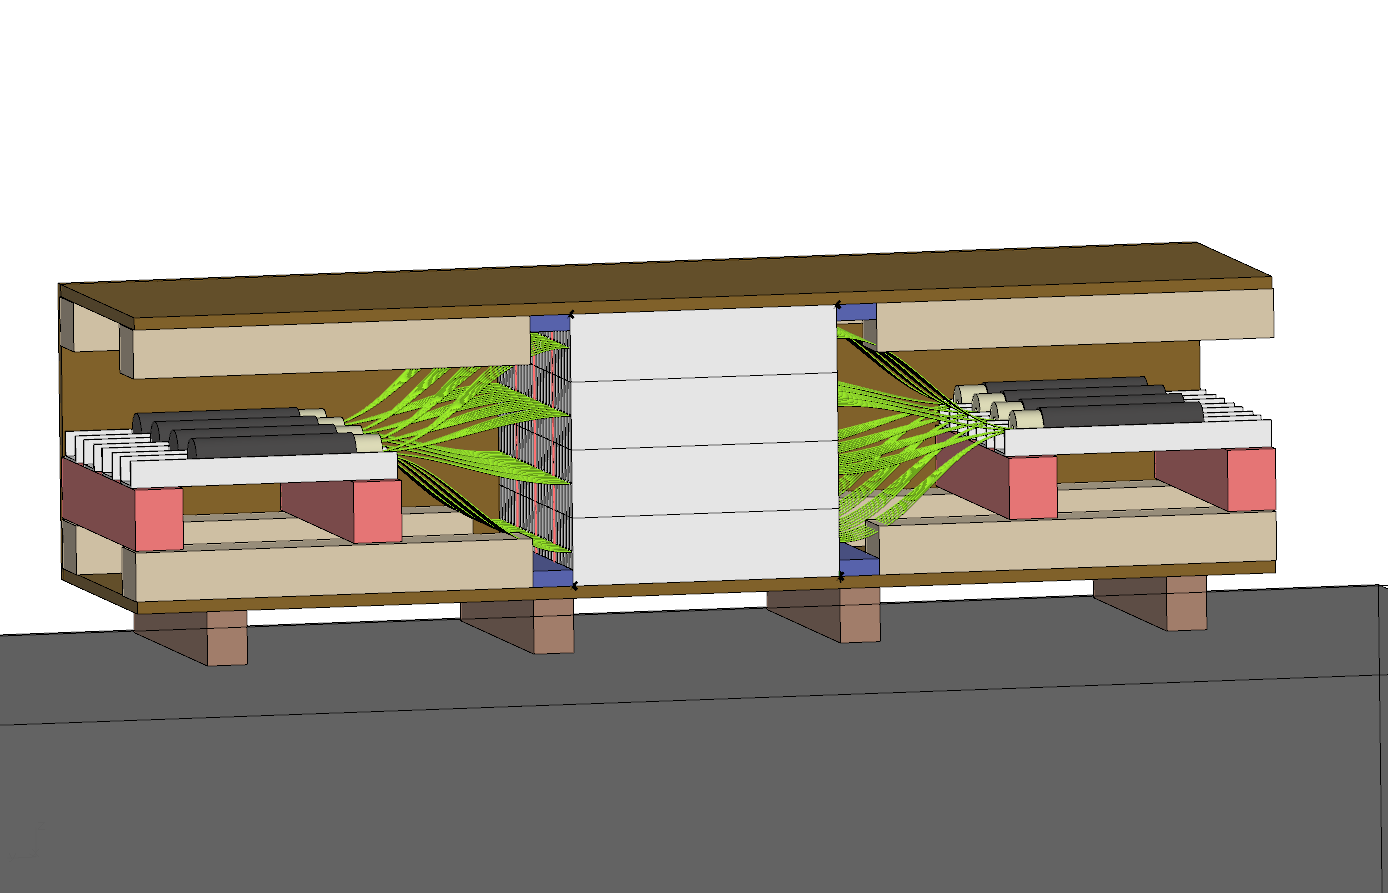
\includegraphics[width=0.6\textwidth]{figure/hayakawa/waku1.png}
\caption{暗箱に固定するための枠の設計}
\end{figure}
\item 暗箱内に設置し前方にコリメータを配置した
\end{itemize}

\begin{figure} [H]
\centering
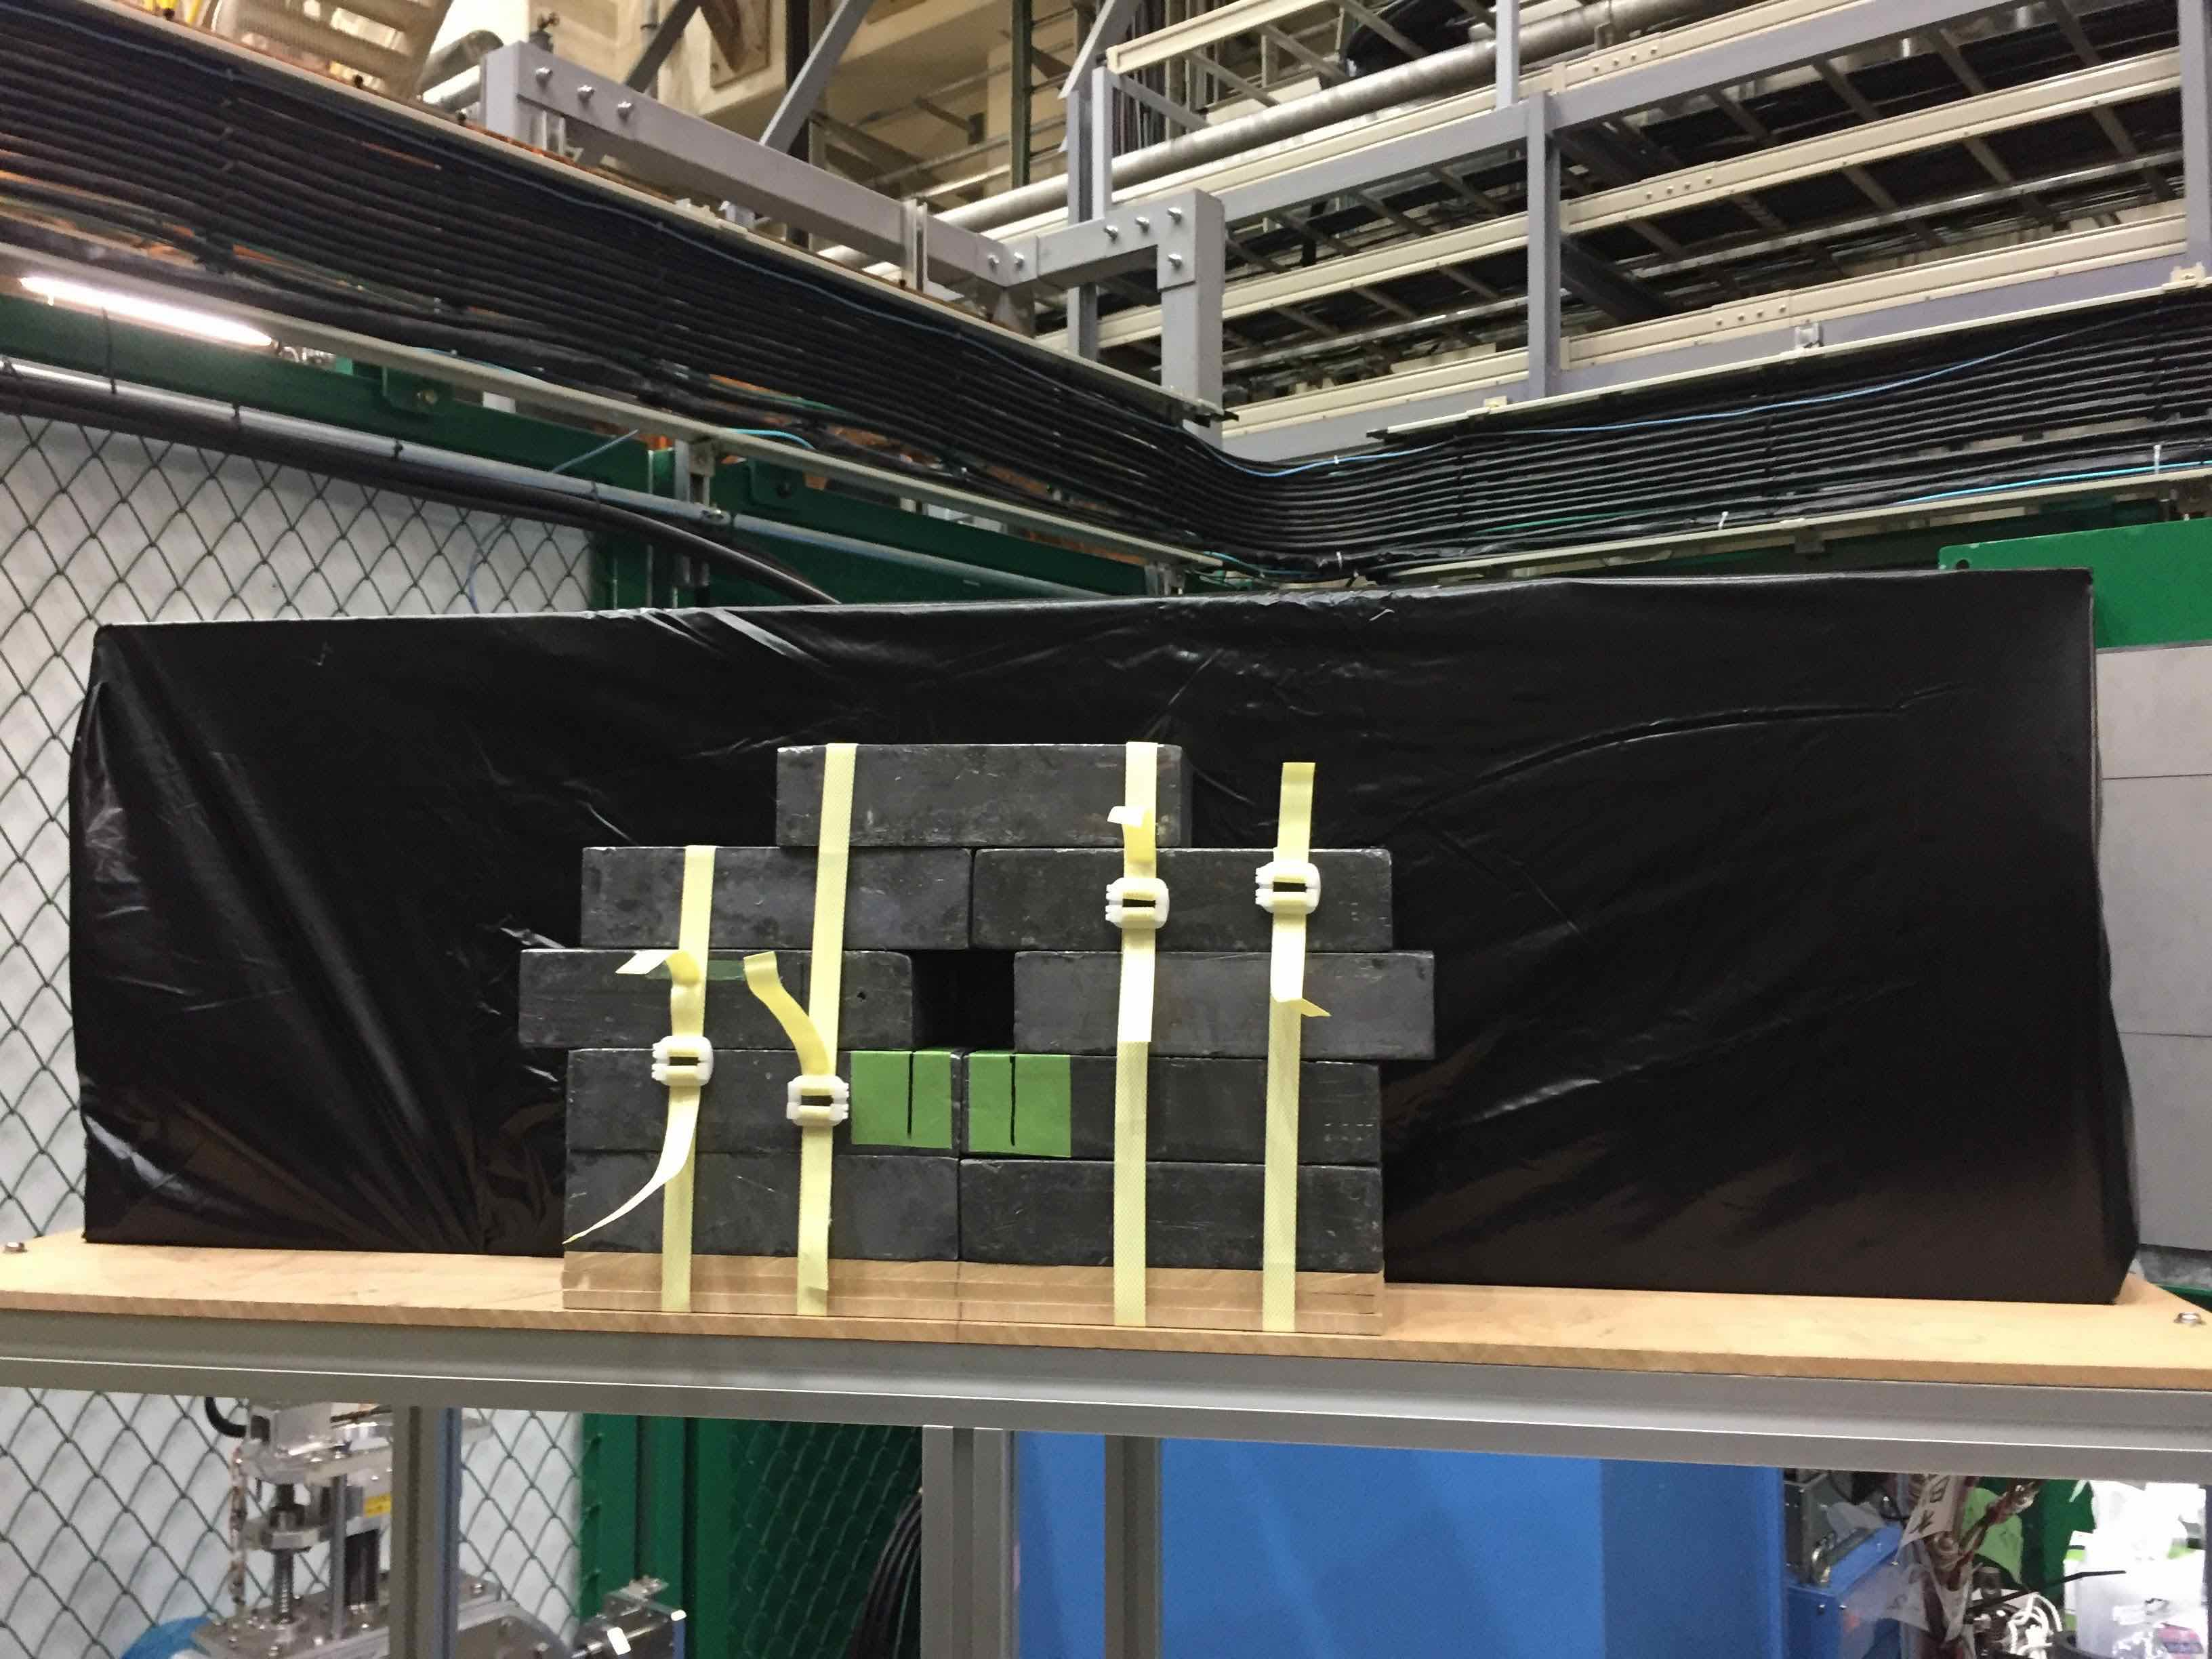
\includegraphics[width=0.6\textwidth]{figure/hayakawa/PS_real.jpg}
\caption{PS 検出器外観}
\end{figure}
\begin{figure}[H]
\centering
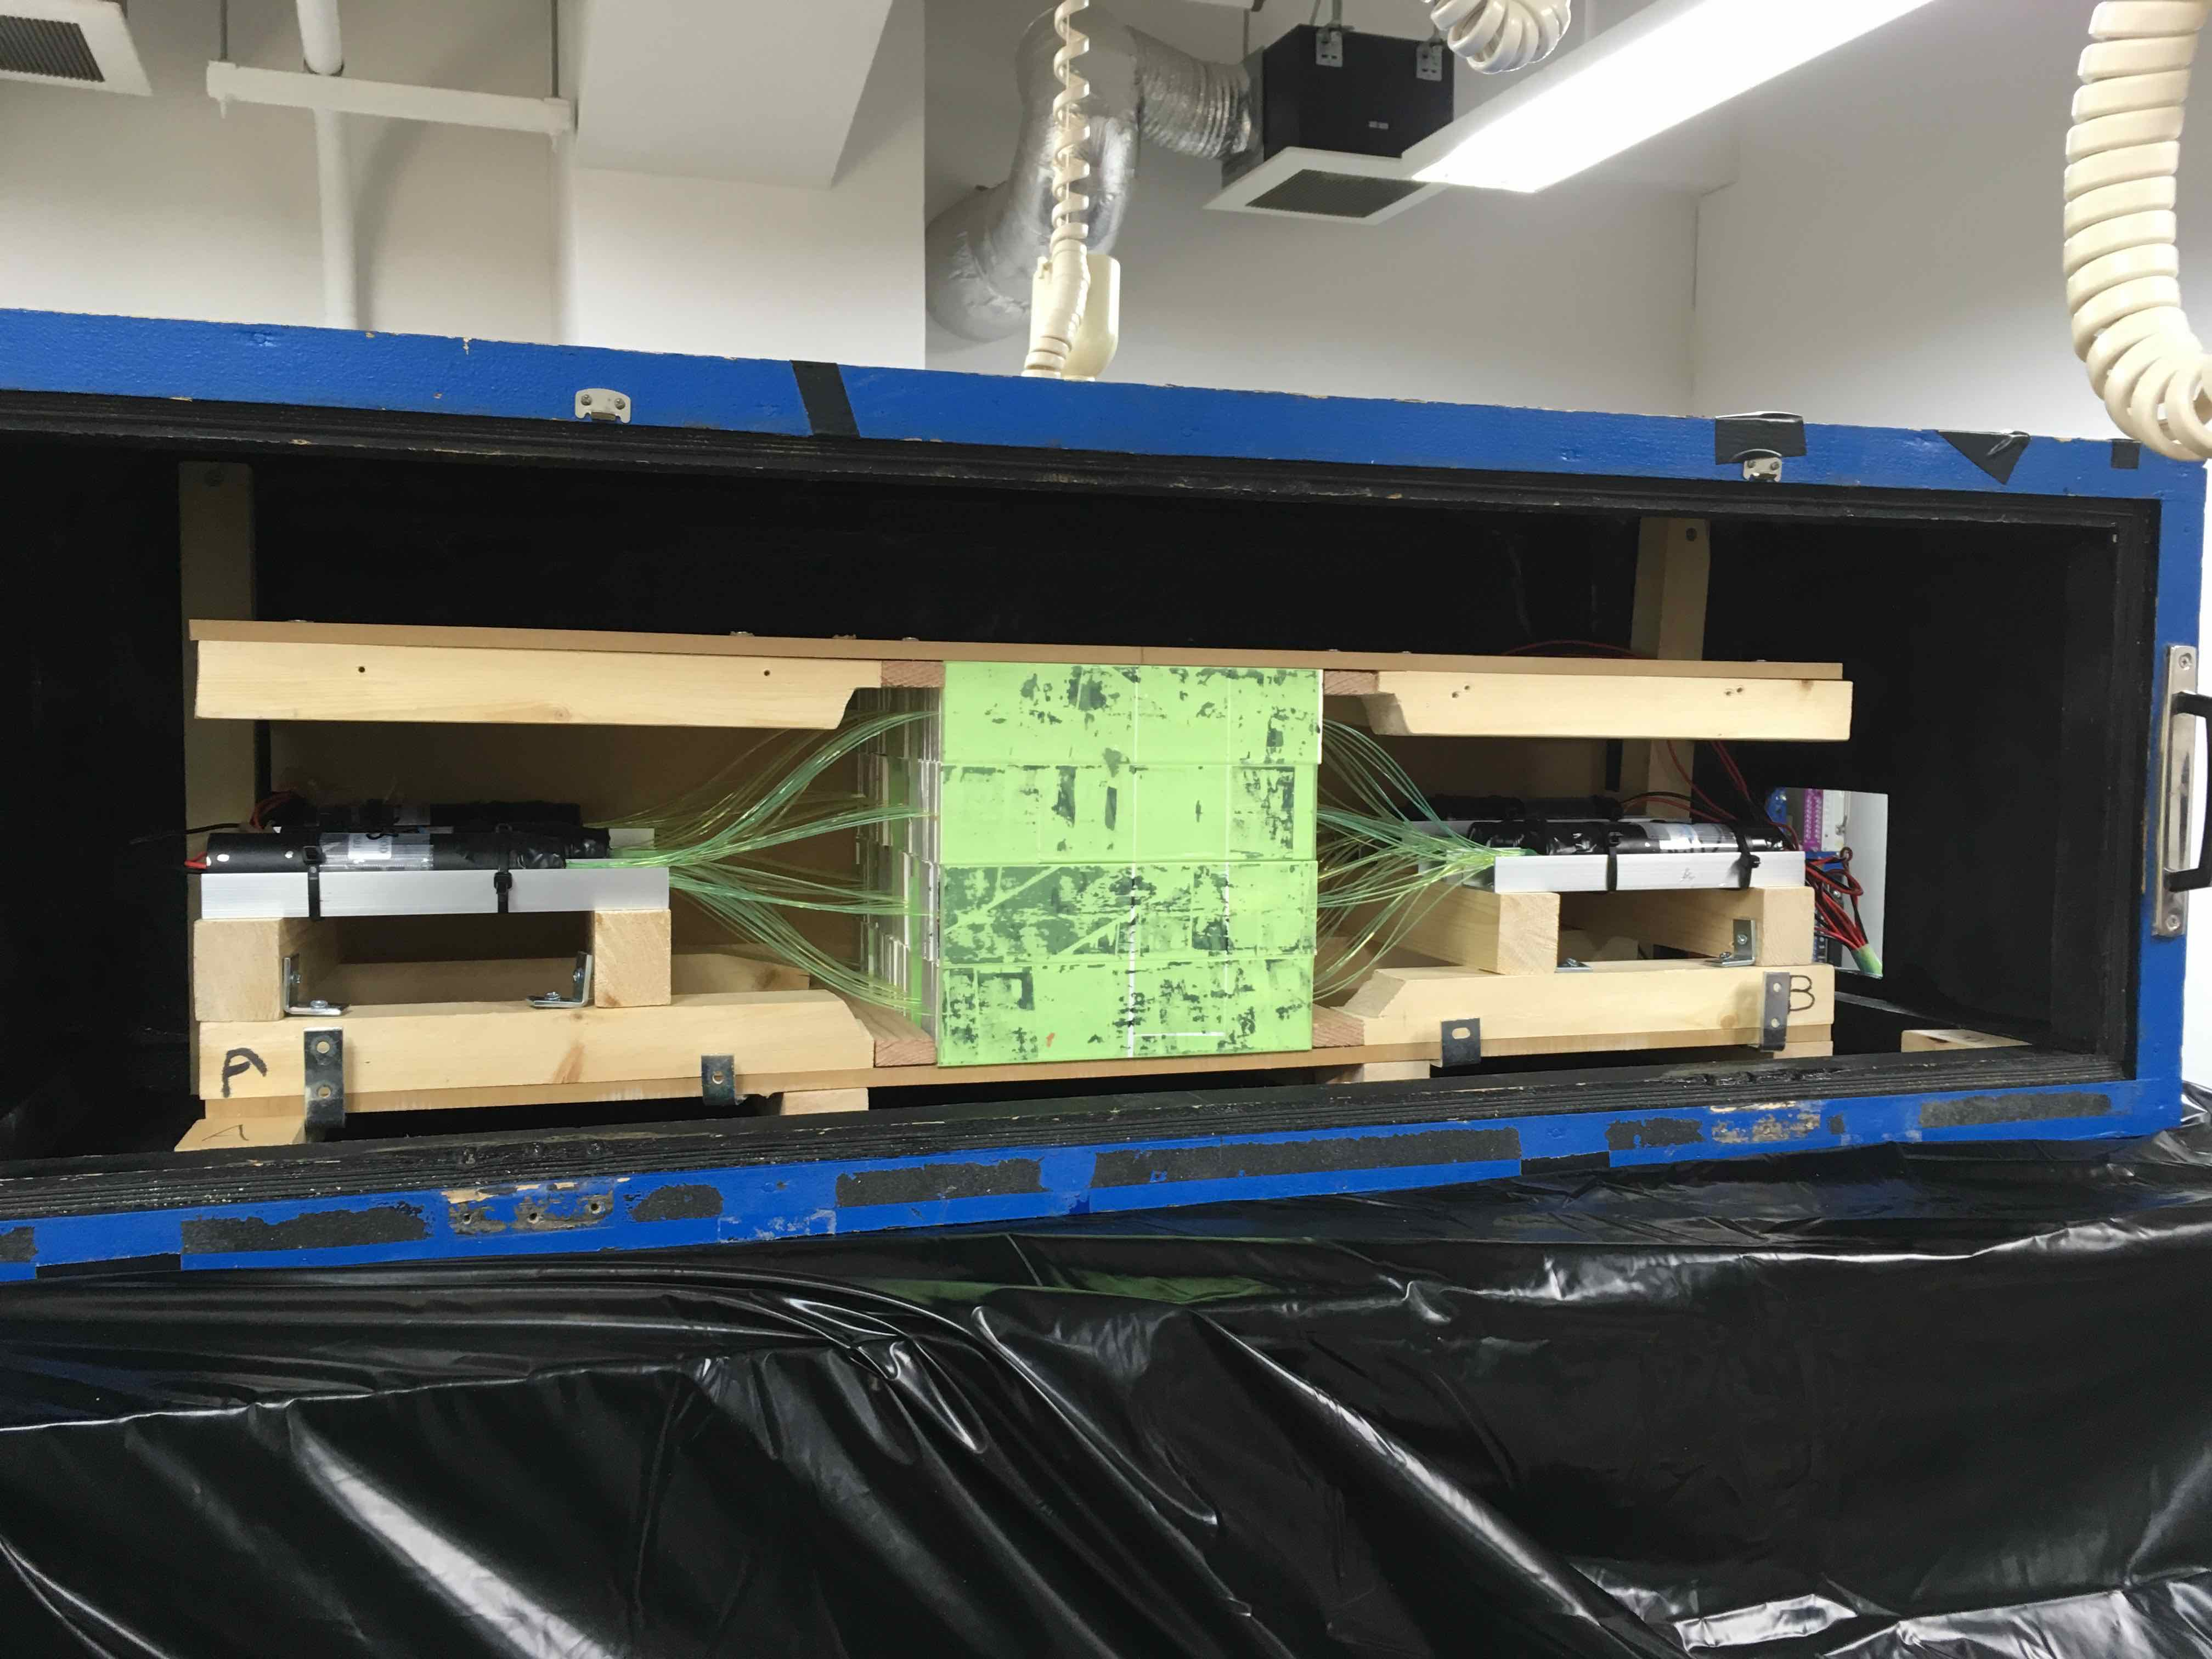
\includegraphics[width=0.7\textwidth]{figure/hayakawa/PS_in.jpg}
\caption{PS検出器内部}
\end{figure}

\subsubsection{NaI 検出器の製作}

$5.6~\mathrm{cm}\times 5.6~\mathrm{cm}\times 15~\mathrm{cm}$ のNaI (Tl) の結晶がPMT に接続されたもの(以下,NaI とよぶ)を$3\times 3$ 個並べ,検出器の前面中央の前には$4~\mathrm{cm} \times 4~\mathrm{cm}$ のプラスチックシンチレータで作ったトリガー用カウンターを設置した.
\begin{figure}
\begin{tabular}{cc}
\begin{minipage}{0.5\hsize}
\centering
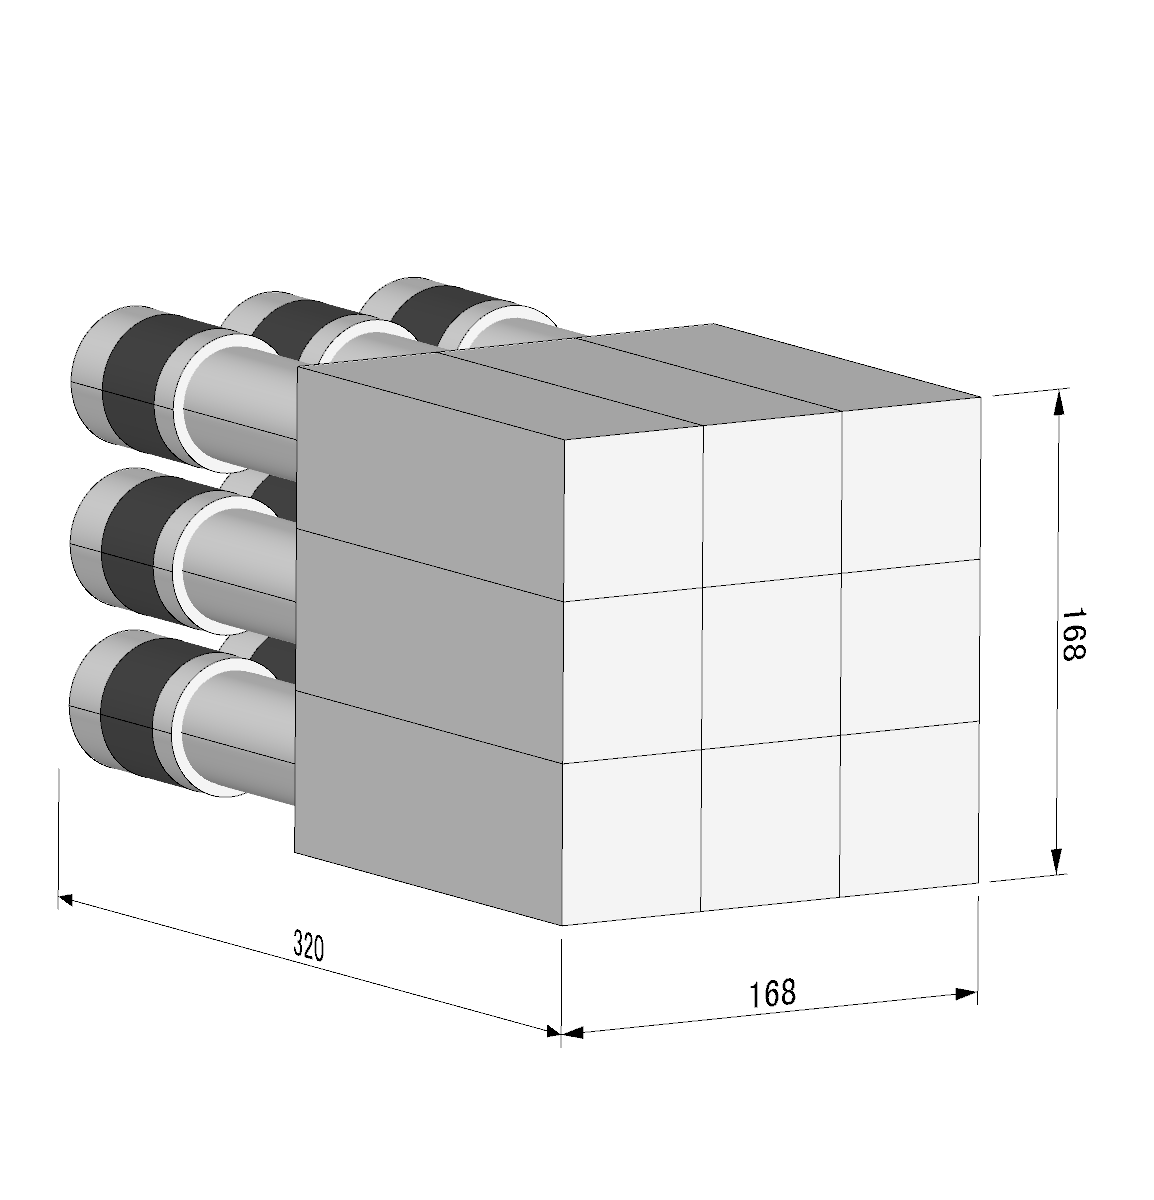
\includegraphics[width=0.8\textwidth]{figure/hayakawa/p6.png}
\caption{NaI 寸法 (mm)}
\end{minipage}
\begin{minipage}{0.5\hsize}
\centering
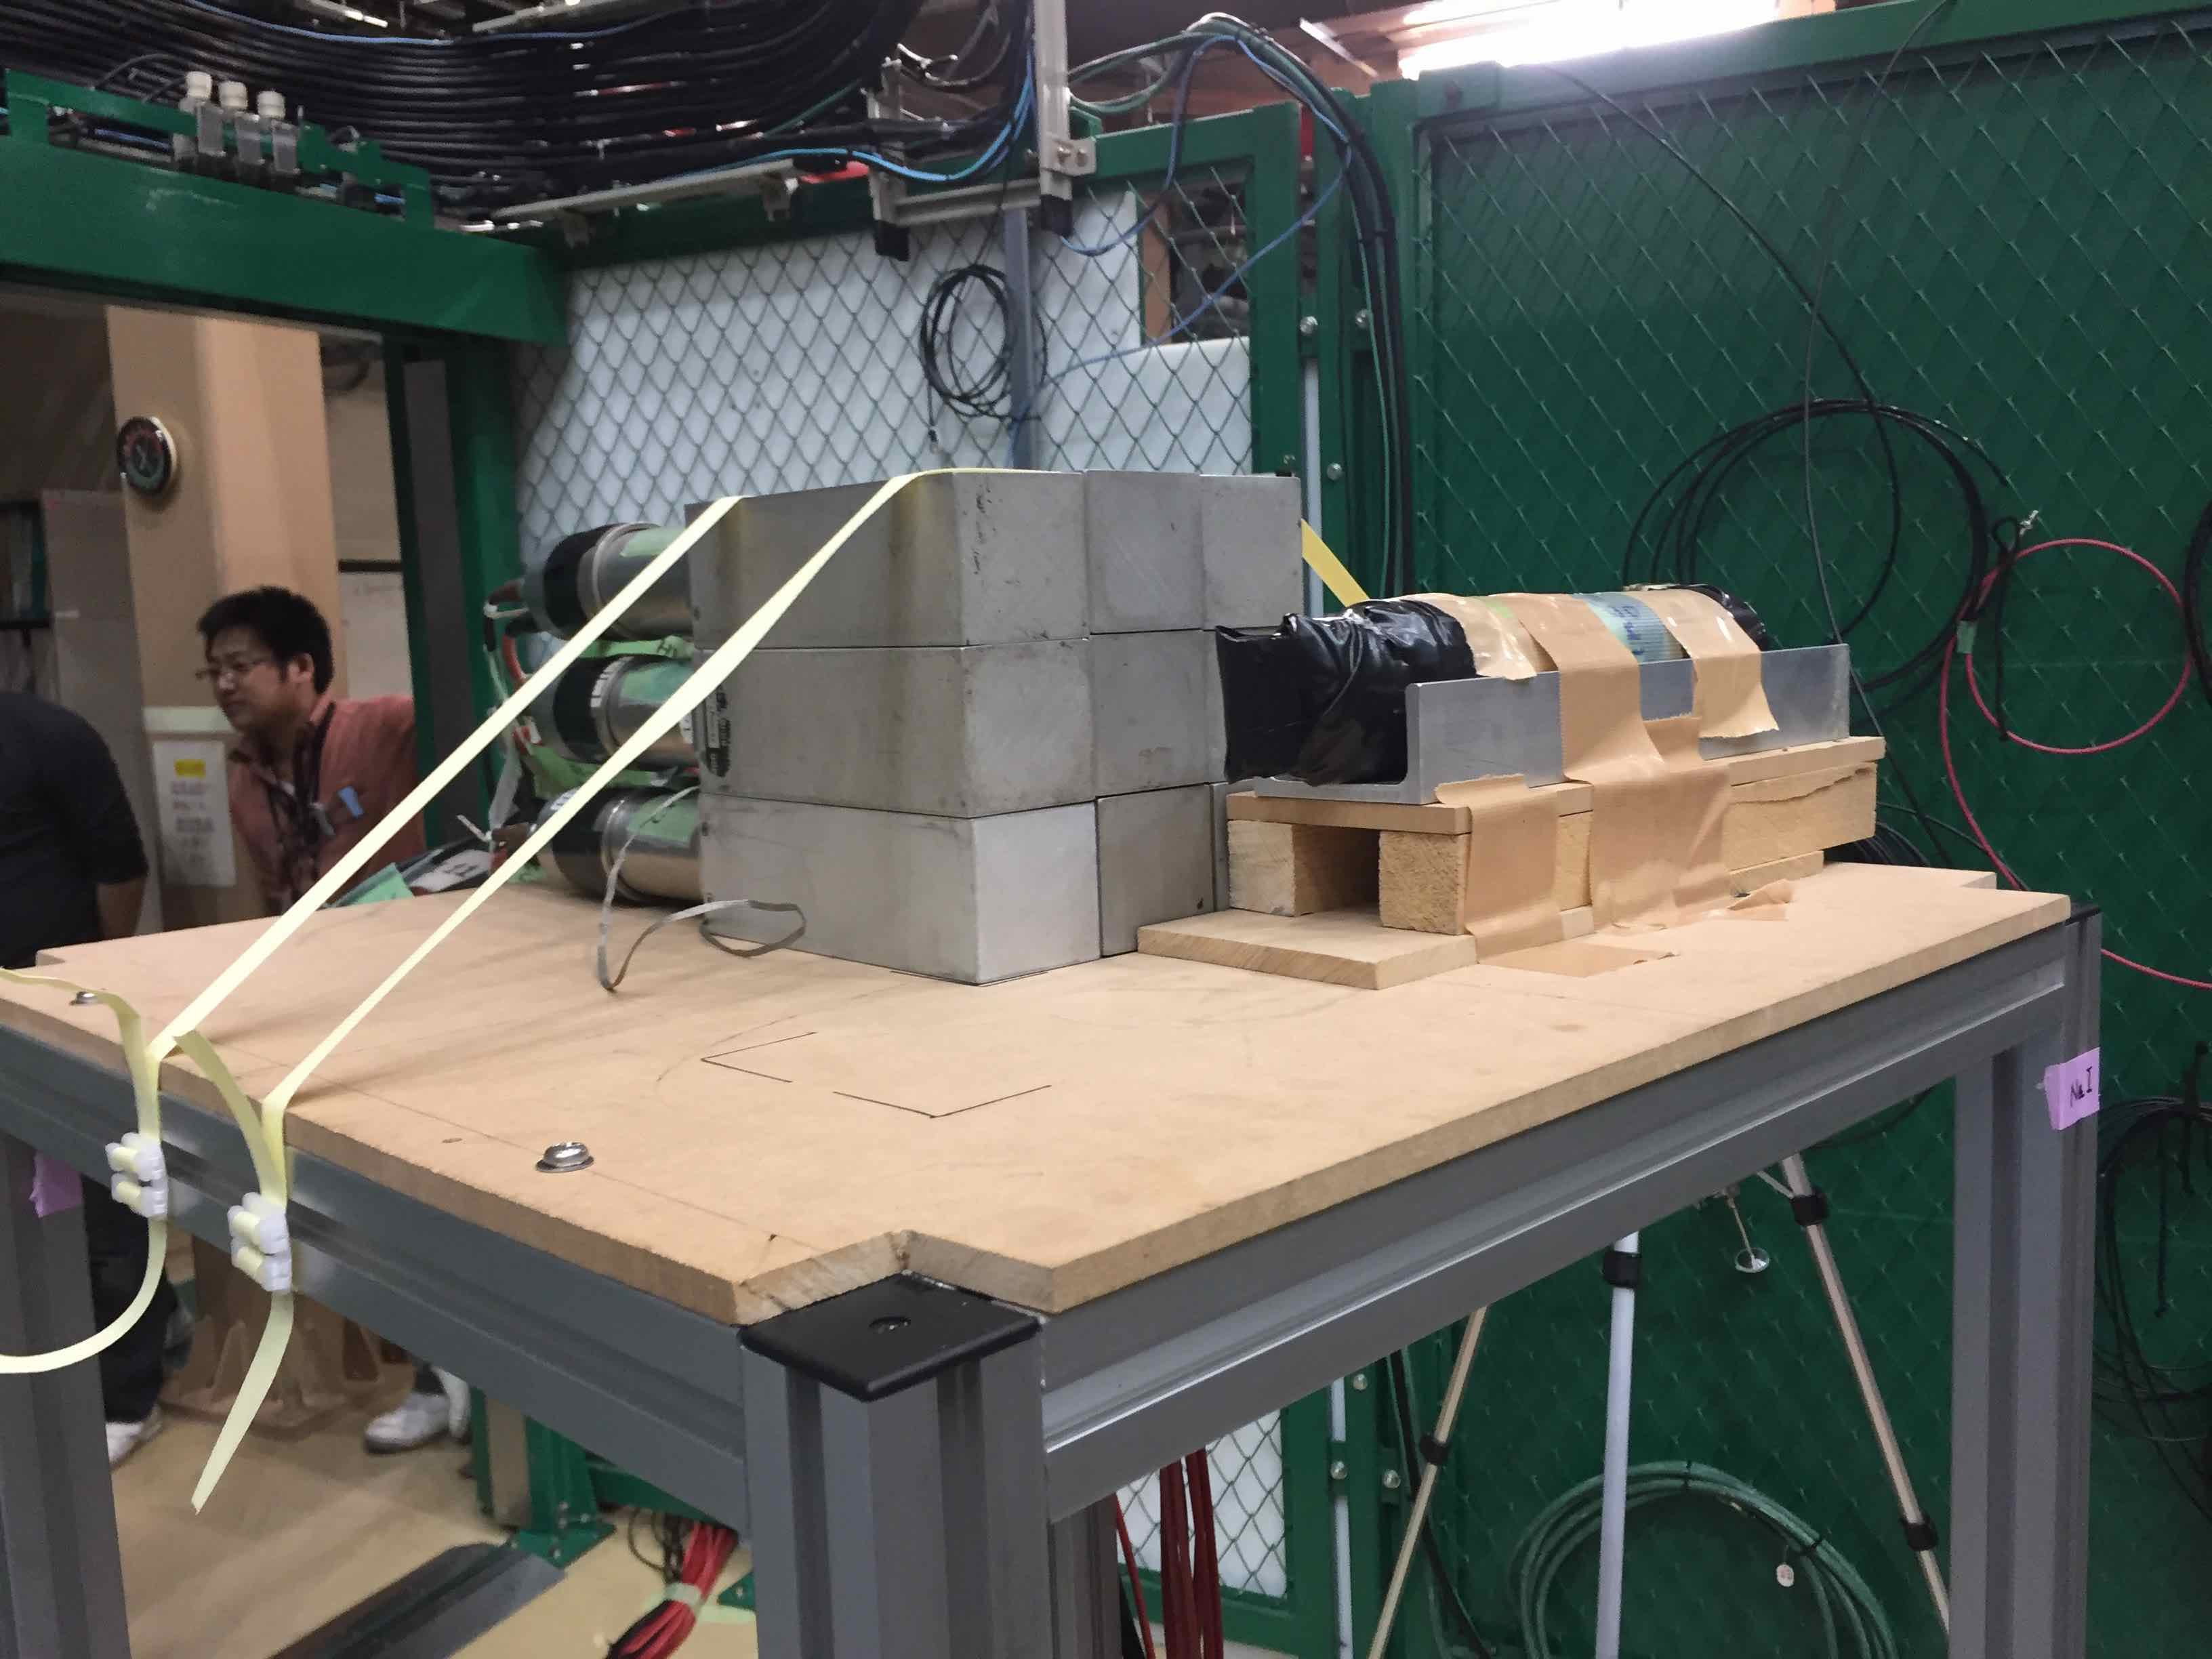
\includegraphics[width=0.8\textwidth]{figure/hayakawa/NaI_real.jpg}
\caption{NaI 外観}
\end{minipage}
\end{tabular}
\end{figure}

\subsection{架台の製作}

ビームの出る高さが地表から$1565~\mathrm{mm}$ なので,検出器を置くためにはその高さに対応した架台が必要であった.そこでアルミフレームの一種であるレコフレームを使用して架台を作成した.アジャスタ付きキャスタを用いることによって高さは微調整可能なように設計した.現場ではレーザーを用いて水平および垂直方向の位置調整を行った.

\begin{figure}[H]
\begin{tabular}{cc}
\begin{minipage}{0.5\hsize}
\centering
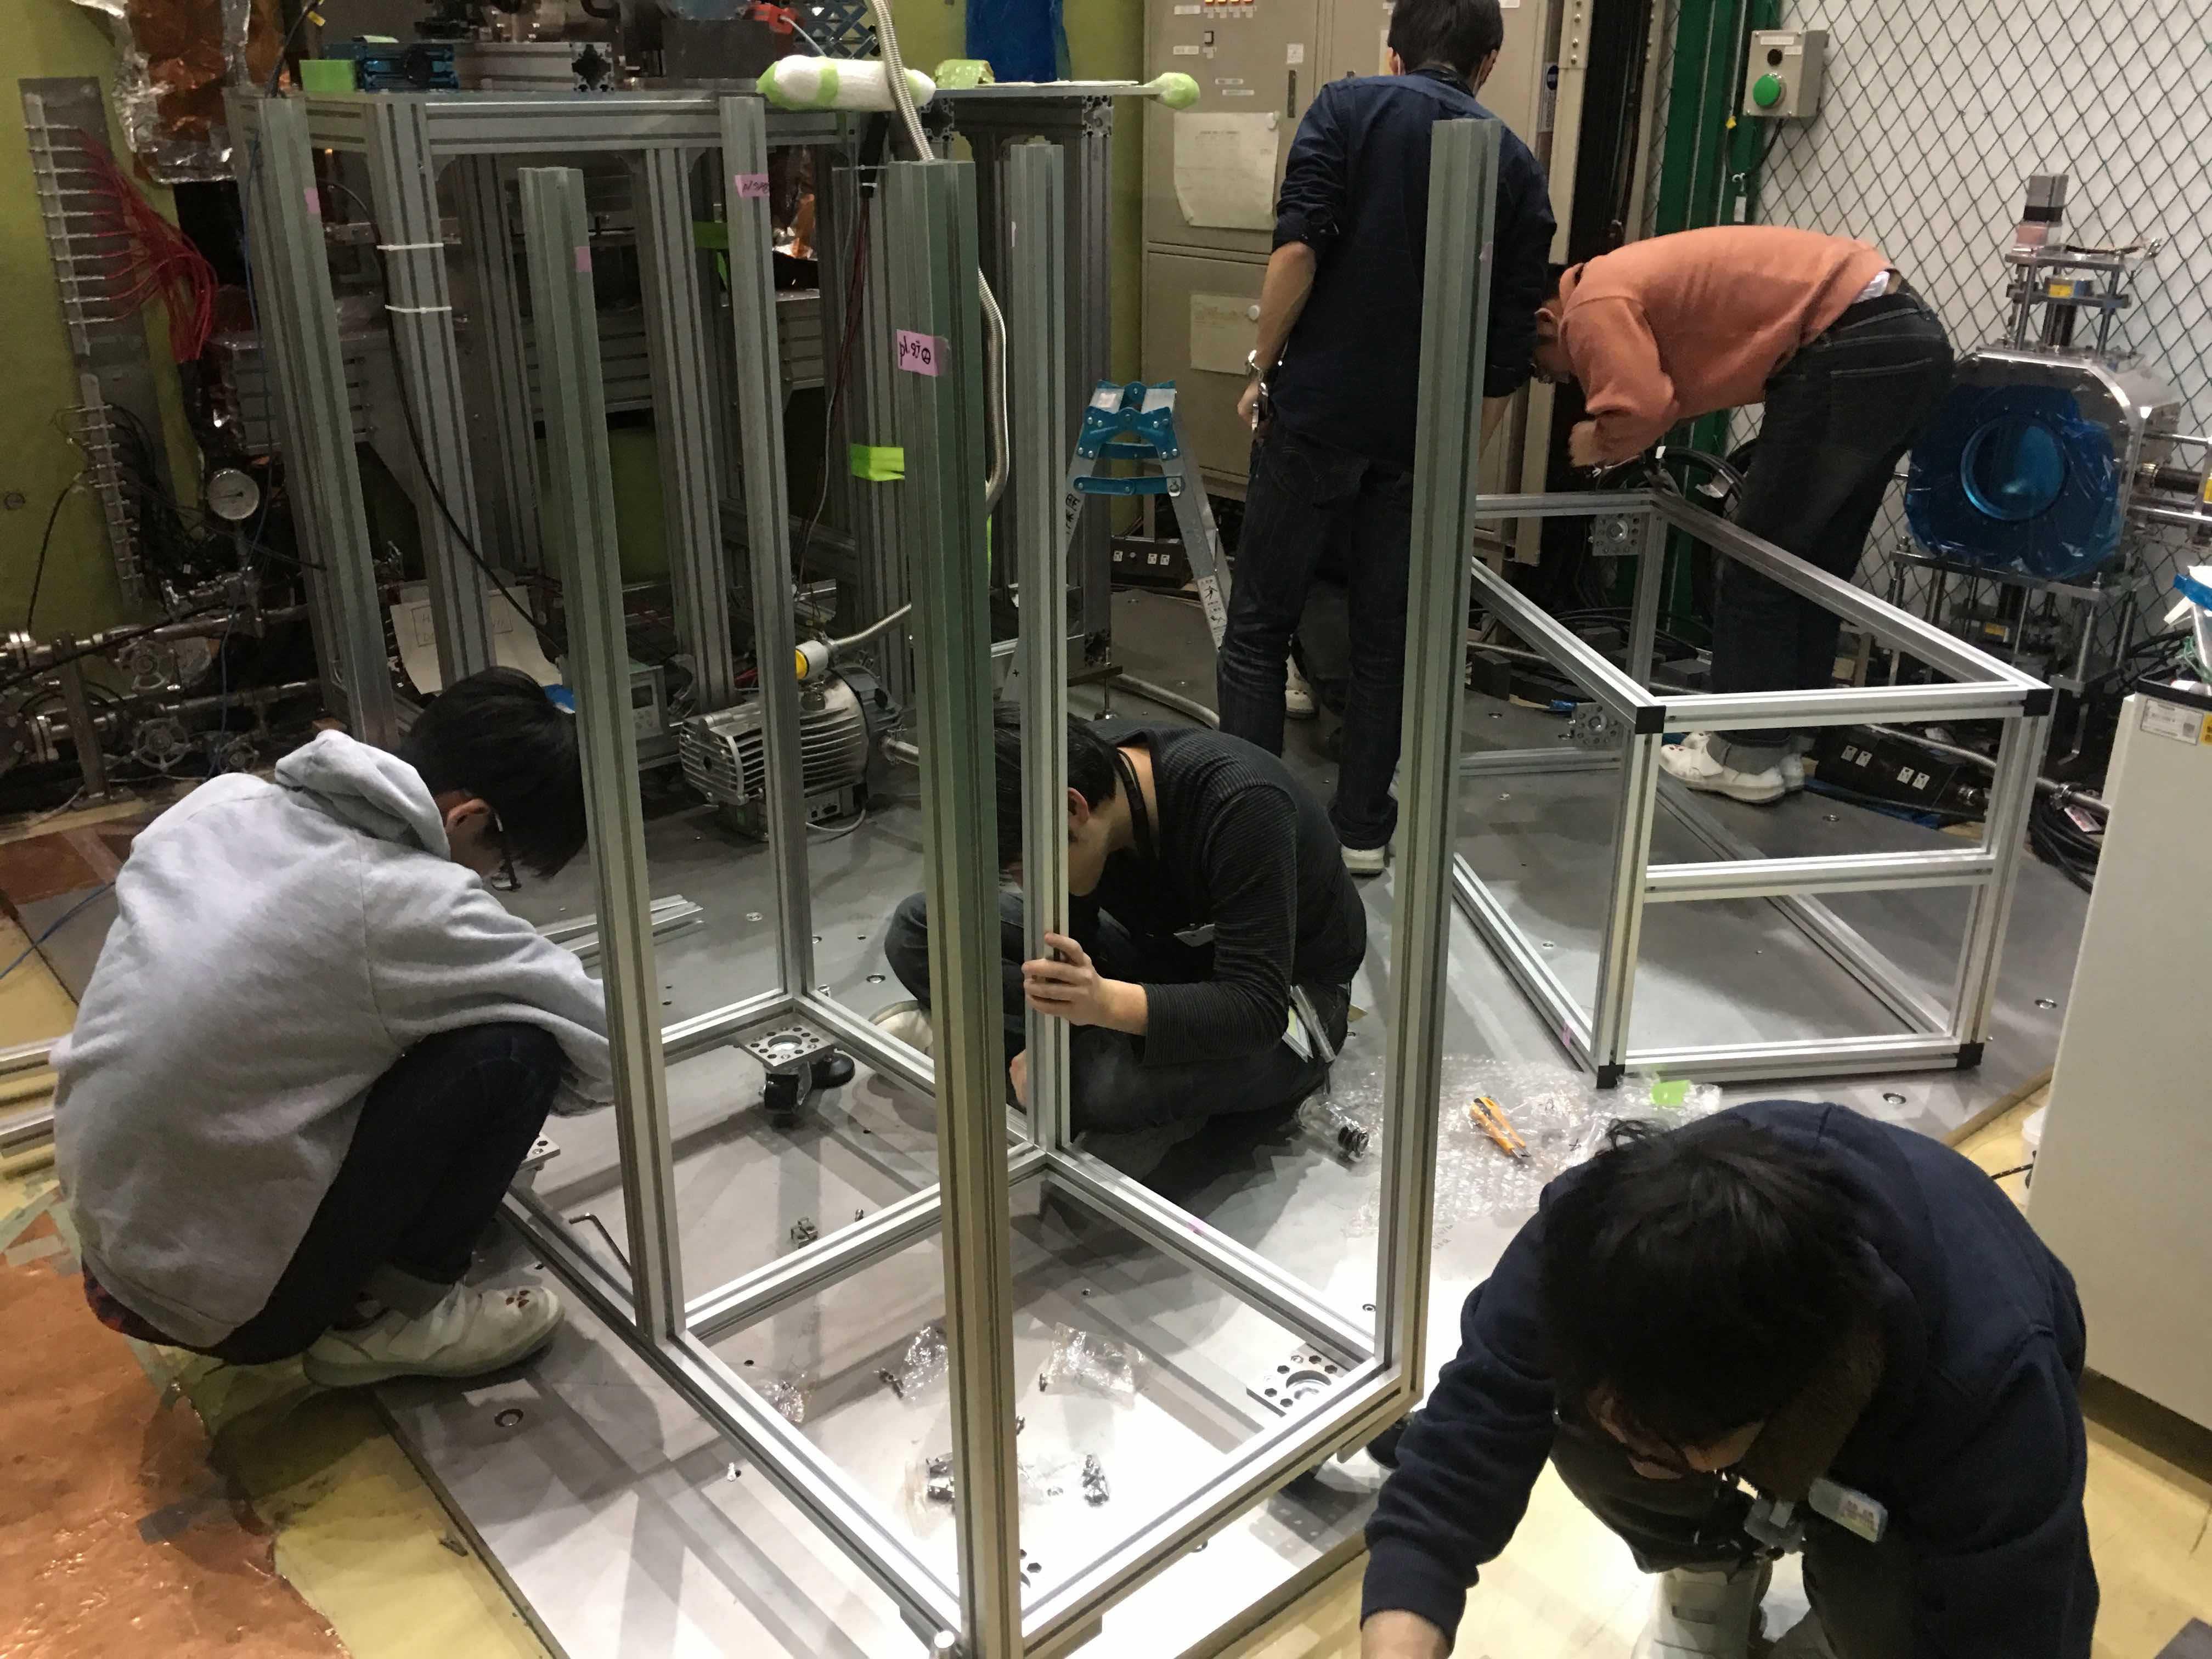
\includegraphics[width=0.9\textwidth]{figure/hayakawa/kadai_setup.jpg}
\caption{架台の組み立て}
\end{minipage}
\begin{minipage}{0.5\hsize}
\centering
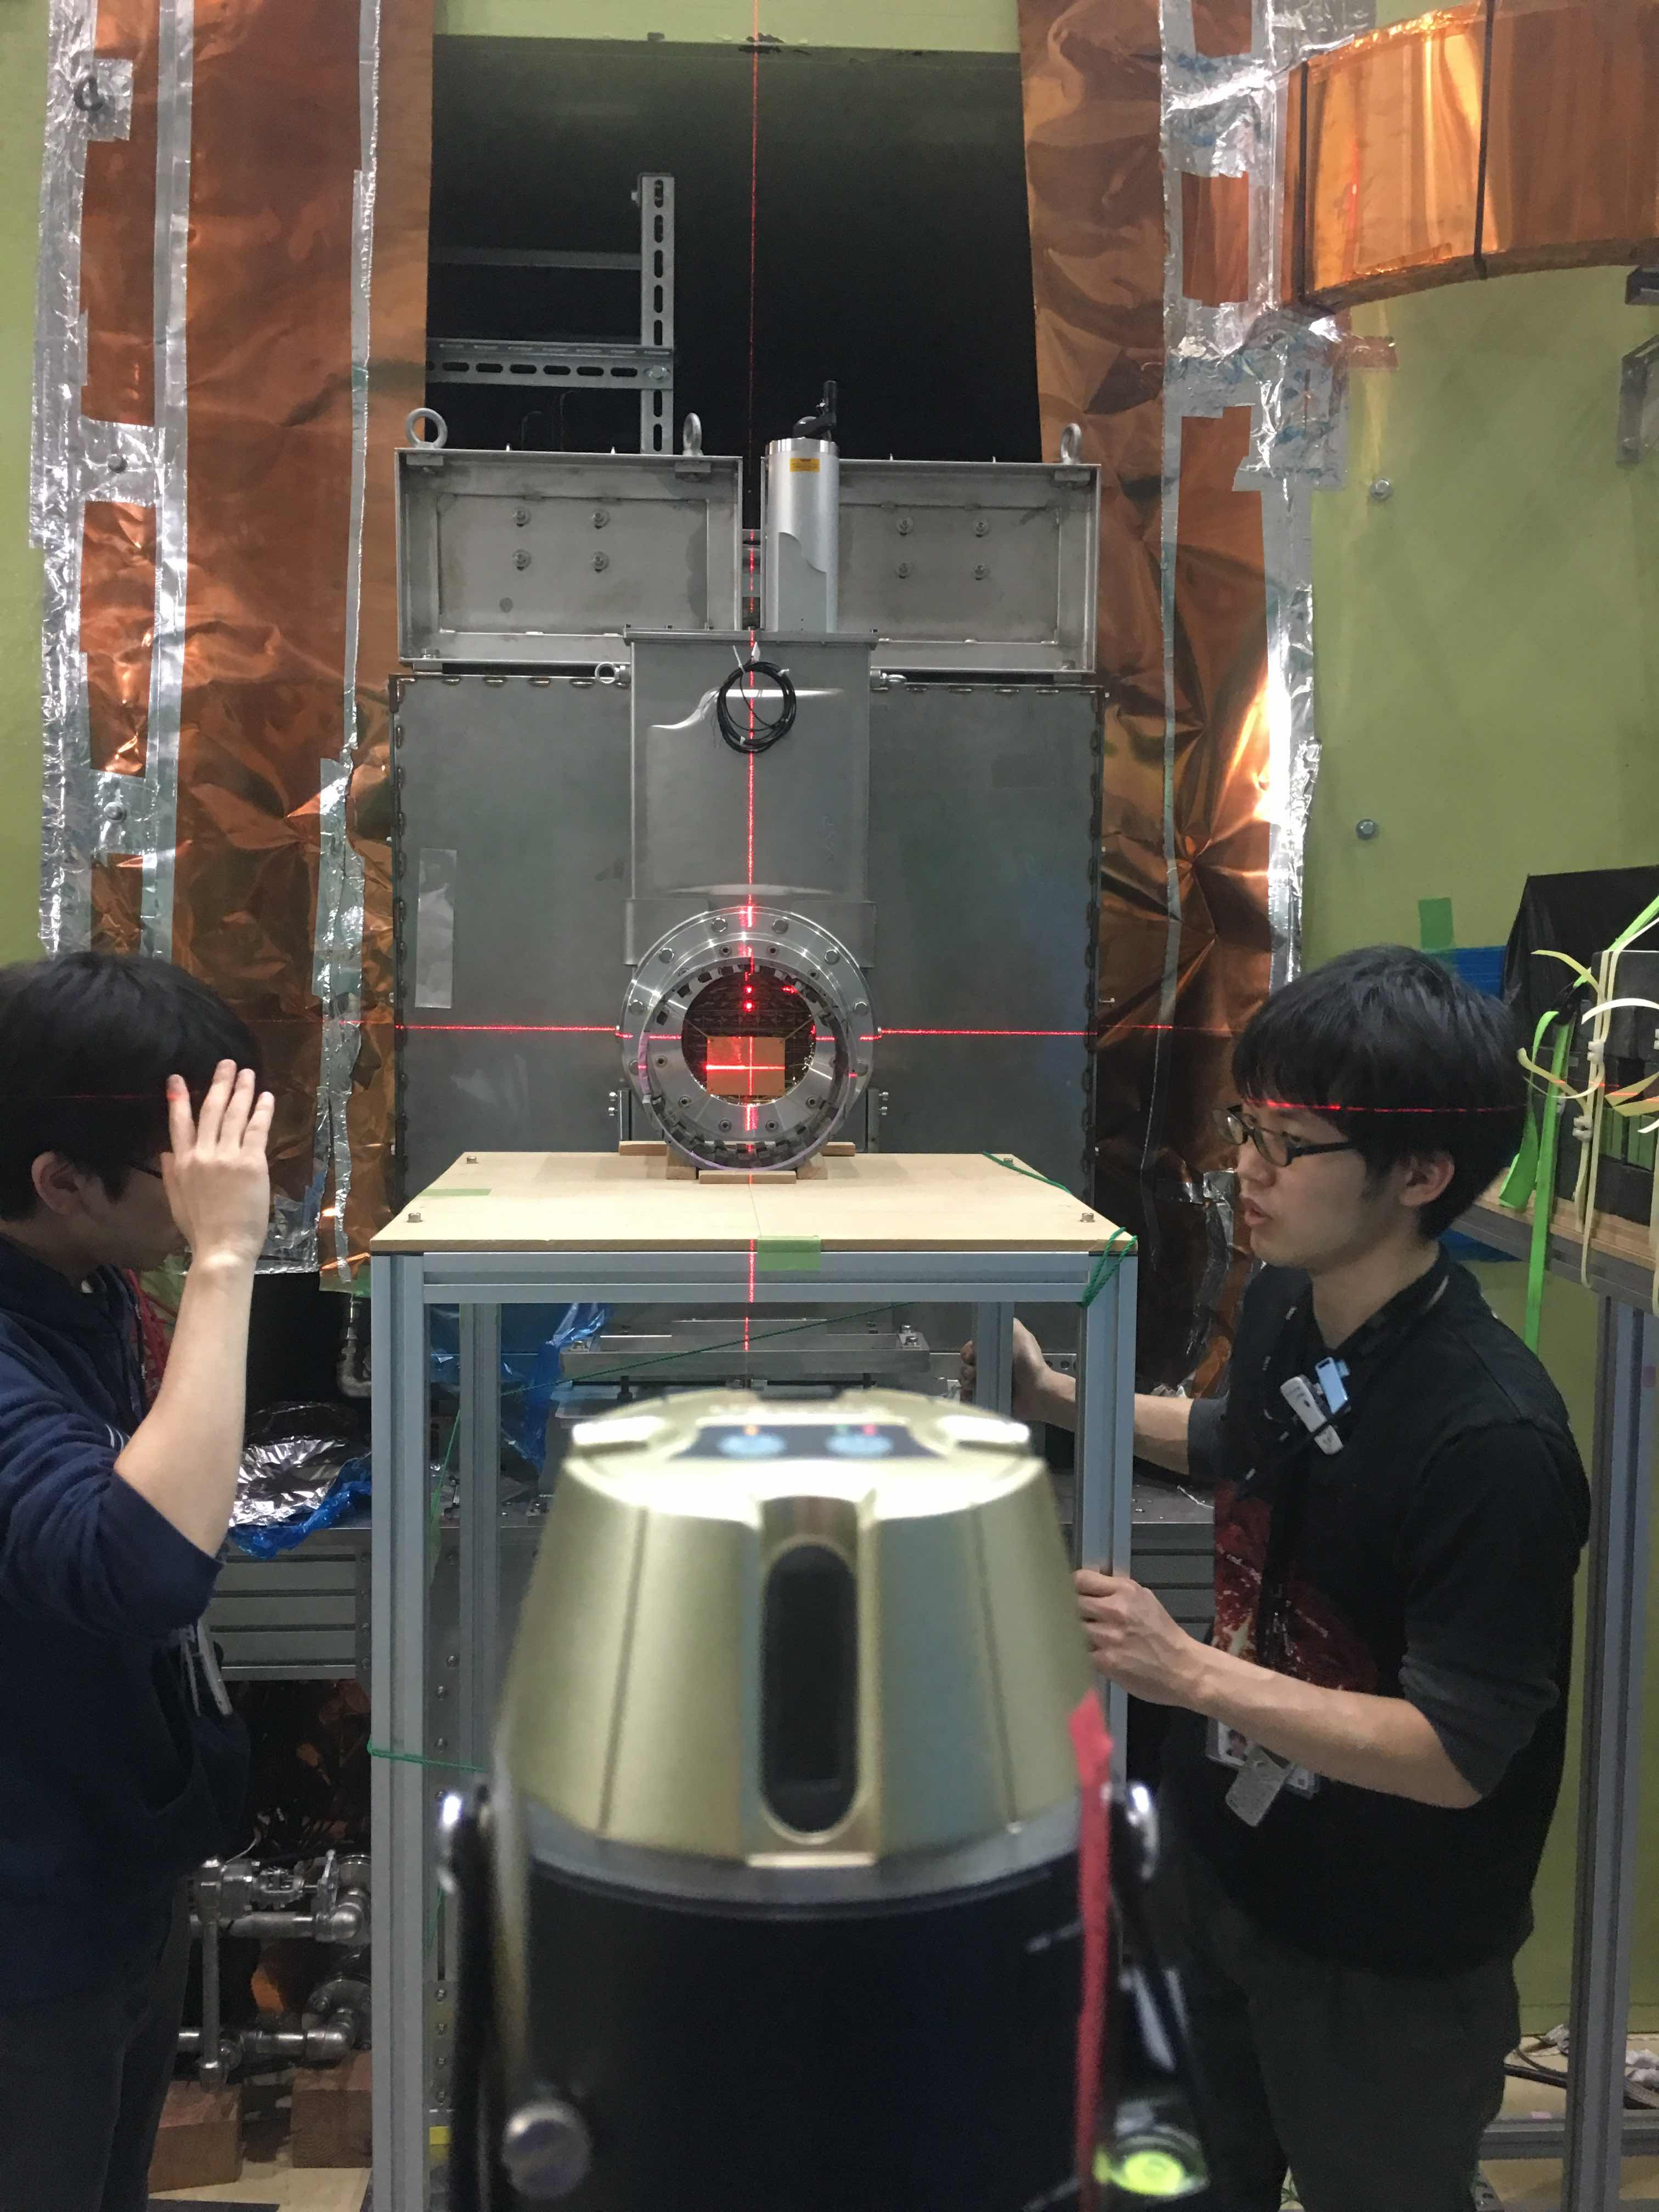
\includegraphics[width=0.9\textwidth]{figure/hayakawa/laser1.jpg}
\caption{レーザーを用いた位置調整}
\end{minipage}
\end{tabular}
 \end{figure}
  
\begin{table}[H]
\caption{3種類の架台の外寸}
\label{tab:kadai}
\centering
\begin{tabular}{|c|c|}\hline
{} &  W $\times$ D $\times$ H (mm)\\ \hline
PS 検出器架台 &  1200 $\times$ 600 $\times$ 1283\\ \hline
NaI 検出器架台 & 600 $\times$ 600 $\times$ 1358 \\ \hline
ターゲット架台 & 600 $\times$ 600 $\times$ 1331 \\ \hline
\end{tabular}
\end{table}

\subsection{Waveform Digitizer}

データ測定については波形をそのまま記録することができるWaveform Digitizer (以下,WFD とよぶ) をPS 検出器およびNaI 検出器用にそれぞれ利用した.測定開始の外部トリガには,加速器ライン側のビームの発射信号を遅延させて陽電子の崩壊の検出のスタートよりわずか手前になるように調整して入力している.

\subsubsection{WFD (CAEN Waveform Digitizer V1721)}
\begin{itemize}
\item 8~channel 8~bit 500~MS/s Digitizer
\item 時間分解能が良いので,主に崩壊寿命測定用のPS の信号に用いた
\end{itemize}
\begin{figure}[H]
\begin{tabular}{cc}
\begin{minipage}{0.5\hsize}
\centering
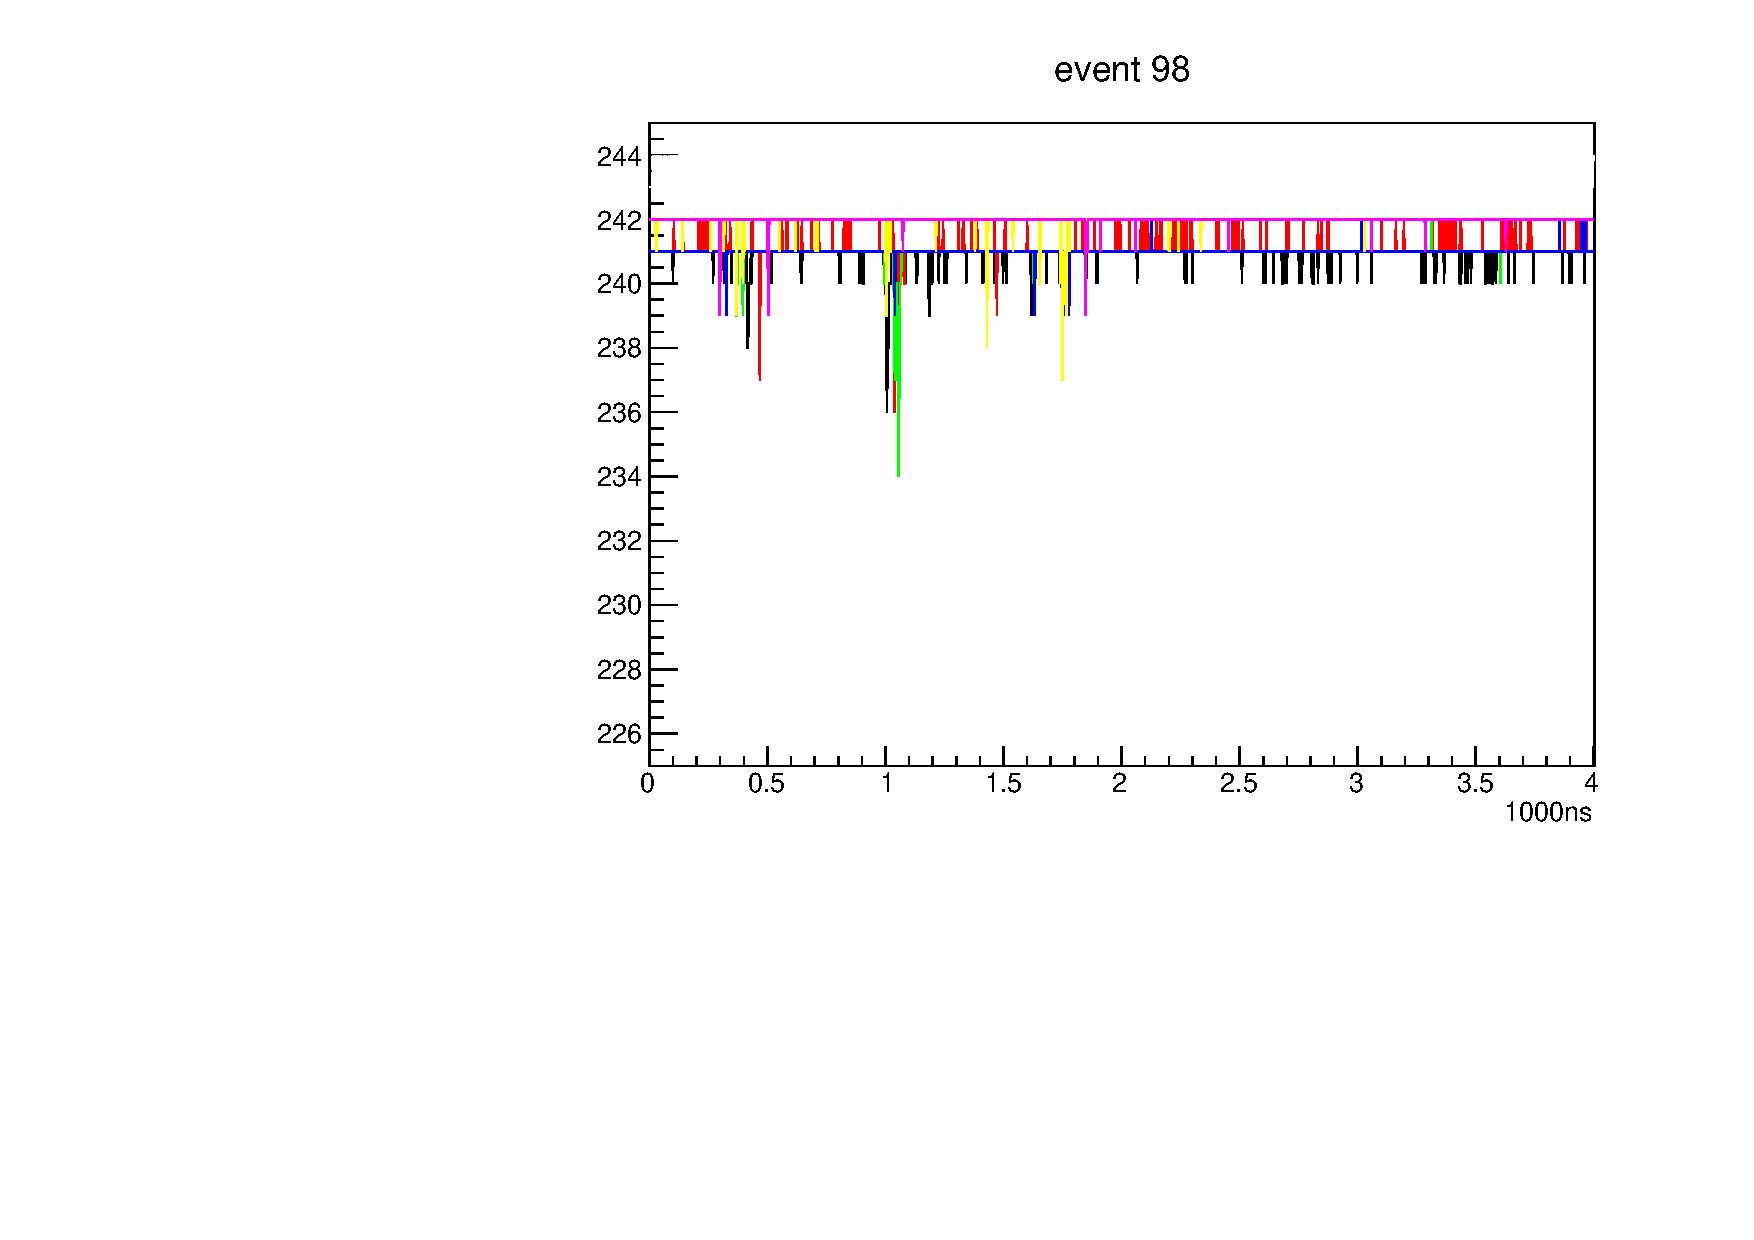
\includegraphics[width=0.8\textwidth,angle=-90]{figure/hayakawa/ps_plot.pdf}
\caption{PS 用のWFD で記録した波形}
\end{minipage}
\begin{minipage}{0.4\hsize}
\centering
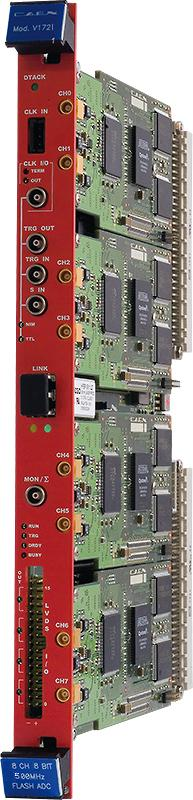
\includegraphics[width=0.2\textwidth]{figure/hayakawa/1095_L.jpg}
\end{minipage}
\end{tabular}
\end{figure}

\subsubsection{WFD (CAEN Waveform Digitizer DT5725)}
\begin{itemize}
\item 8~channel 14~bit 250~MS/s Digitizer
\item エネルギー分解能が良いので,主にエネルギー測定用のNaI 検出器の信号の記録に用いた
\item 9~本のNaI に対して8~チャンネルとチャンネル数が不足していたので,アナログ信号を合成して入力した
\end{itemize}
\begin{figure}[H]
\begin{tabular}{cc}
\begin{minipage}{0.5\hsize}
\centering
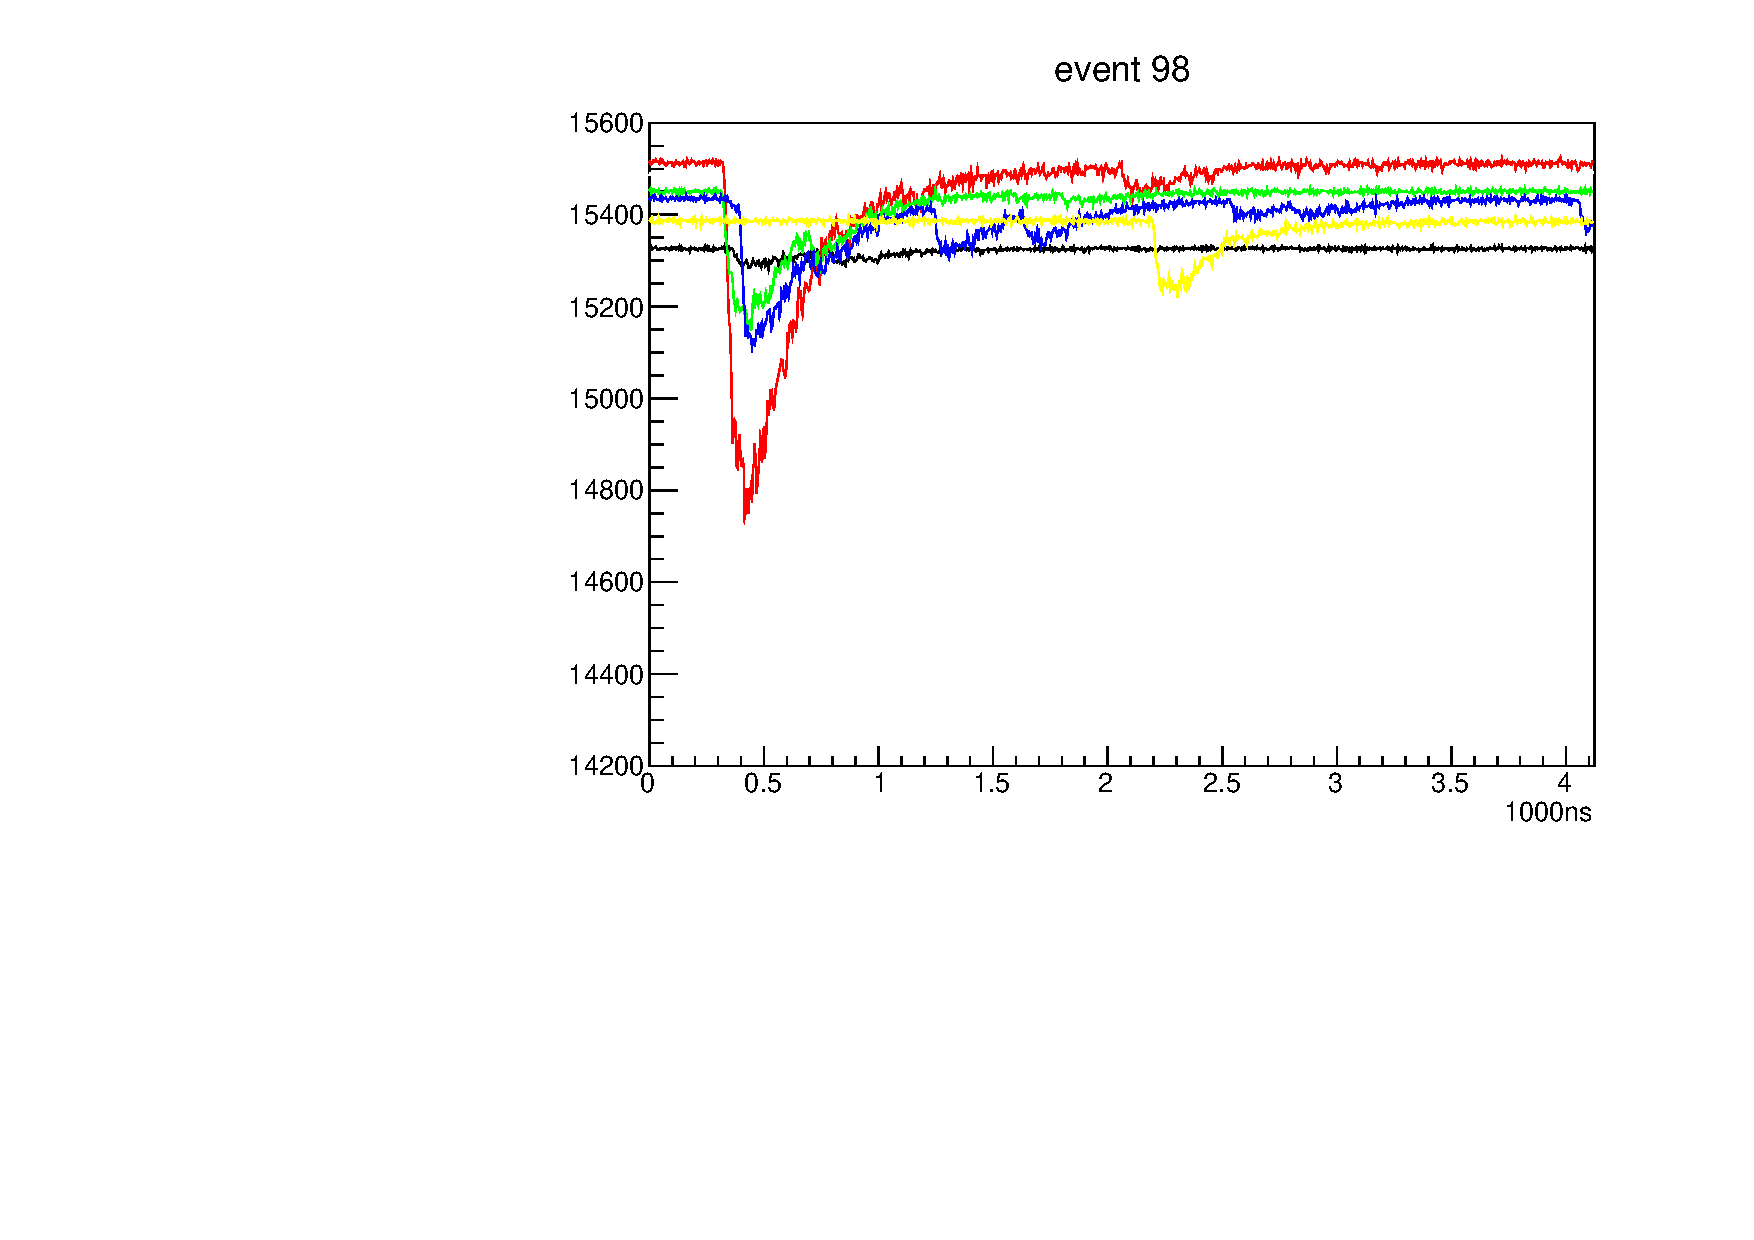
\includegraphics[width=0.8\textwidth,angle=-90]{figure/hayakawa/NaI_plot.pdf}
\caption{NaI 用のWFD で記録した波形}
\end{minipage}
\begin{minipage}{0.4\hsize}
\centering
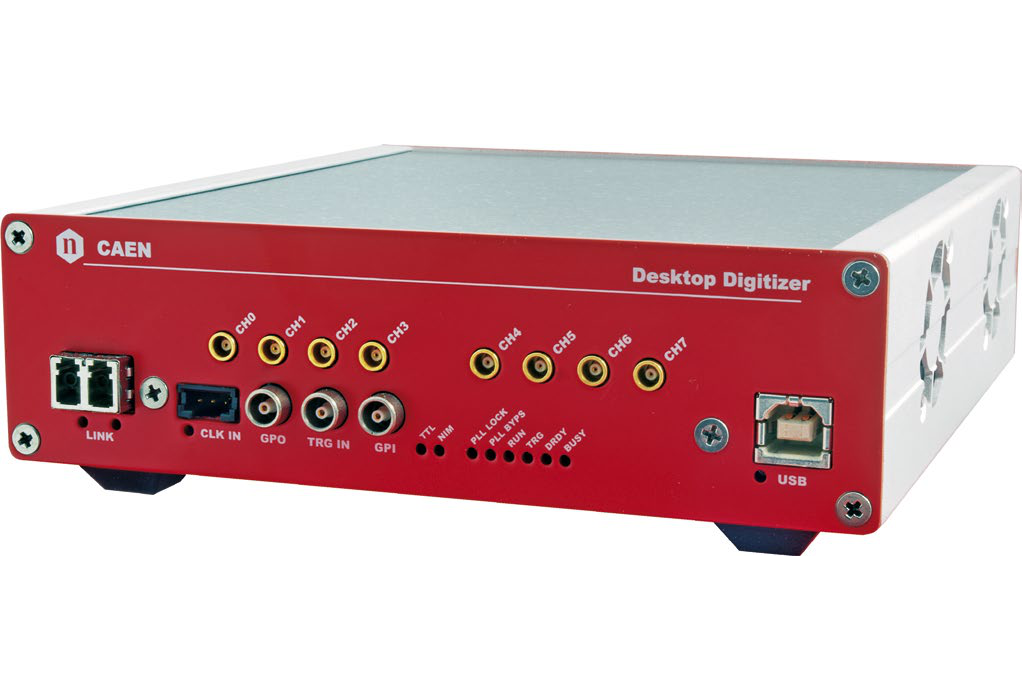
\includegraphics[width=0.6\textwidth]{figure/hayakawa/DT5725_L.png}
\end{minipage}
\end{tabular}
\end{figure}

%\end{document}
